\documentclass[geometry_main]{subfiles}

\begin{document}

\setcounter{chapter}{1}

\chapter{多様体}

集合の\hyperref[ax.topo]{位相}とは,異なる点同士の「近さ」の概念を定式化したものと言える.その意味で,集合 $M$ の上に位相を定めて\hyperref[ax.topo]{位相空間} $(M,\, \mathscr{O})$ を作れば,$M$ のことを図形と呼べるであろう.
さらに $M$ に次のような要請を与える:
\begin{itemize}
	\item $M$ はHausdorff空間である
	\item $M$ は\textbf{局所的に}我々のよく知る $\mathbb{R}^n (\mathbb{C}^n)$ と同一視できる
\end{itemize}
第一の要請により,点列の収束先が一意に定まることが保証される.
第二の要請は,$M$ 上の点を座標で表示できることを意味する.

\section{位相多様体}

\subsection{定義}

\begin{mydef}[label=def.topomani, breakable]{位相多様体}
	\hyperref[def:second-countable]{第2可算}な\hyperref[def:separation]{Hausdorff空間} $(M,\, \mathscr{O}_M)$ が
	$n$ 次元\textbf{位相多様体} (topological manifold) であるとは,
	任意の点 $p \in M$ に対して
	\begin{itemize}
		\item $p$ の\hyperref[def:neighborhood]{開近傍}$p \in U \subset M$
		\item $\mathbb{R}^n$ の開集合 $\varphi(U) \subset \mathbb{R}^n$
		\item \hyperref[def.homeo]{同相写像}
		$\varphi \colon U \xrightarrow{\approx} \varphi(U)$
	\end{itemize}
	の3つが存在することを言う.
\end{mydef}
少し技術的な話をすると,上述の定義において開集合 $\varphi(U) \subset \mathbb{R}^n$ を\hyperref[def:epsilon-neighbourhood]{開球} $B_{\varepsilon} \bigl(0\bigr) \subset \mathbb{R}^n\; (\varepsilon > 0)$ か,もしくは $\mathbb{R}^n$ そのものに置き換えても同値な定義が得られる
\footnote{$\forall p \in M$ に対して定義\ref{def.topomani}の3つ組が与えられたとする.平行移動により $\varphi(p) = 0 \in \mathbb{R}^n$ を仮定して良い.
このとき\hyperref[prop.opdet]{開集合の性質}から $\varphi(p) \in B_\varepsilon (0) \subset \varphi(U)$ を充たす $\varepsilon > 0$ が存在するので
$M$ の開集合\footnote{$\varphi$ の\hyperref[def.continuous]{連続性}より $\varphi^{-1} \bigl(B_\varepsilon (0) \bigr)$ は $M$ の開集合.} $\varphi^{-1} \bigl(B_\varepsilon (0) \bigr) \subset M$ と $B_\varepsilon(0) \subset \mathbb{R}^n$ と $\varphi$ の制限 $\varphi|_{\varphi^{-1}\bigl(B_\varepsilon(0)\bigr)}$ (これも同相写像になっている)が定義\ref{def.topomani}の3つ組に相当するものになる.
$B_\varepsilon (0) \approx \mathbb{R}^n$ は,例えば連続写像 $x \lmto \frac{x}{\varepsilon-\abs{x}}$ が同相写像になっている.
}.

$\mathbb{R}^n$ との局所的な同相の構造を入れたことで,位相多様体 $M$ 上の点を座標表示することができるようになる.
\begin{mydef}[label=def.localcoord, breakable]{局所座標}
	$n$次元位相多様体 $\phase{M}$ を与える.
	$M$ 上の任意の点 $p \in M$ をとり,
	$p$ の\hyperref[def:neighborhood]{開近傍} $p \in U \subset M$ であって $\mathbb{R}^n$ の開集合 $\varphi(U) \subset \mathbb{R}^n$ との\hyperref[def.homeo]{同相写像} $\varphi \colon U \xrightarrow{\approx} \varphi(U)$ が存在するものをとる.
	このとき,
	\begin{itemize}
		\item $U \in \mathscr{O}_M$ を点 $p$ の\textbf{座標近傍} (coordinate neighborhood) と呼ぶ.
		\item 組 $(U,\, \varphi)$ のことを\textbf{チャート} (chart),もしくは\textbf{局所座標系}と呼ぶ.
		\item 任意の点 $q \in U$ に対して,$q$ が $\varphi$ によって写像された行き先
		\begin{align}
			\varphi(q) = \bigl(\, x^1(q),\, x^2(q),\, \dots ,\, x^n(q) \,\bigr) \in \mathbb{R}^n
		\end{align}
		のこと\footnote{添字が上付きになっている理由は後ほど明らかになる.}を点 $q$ の\textbf{局所座標} (local coordinate) と呼ぶ.
		\item $\mu = 1,\, \dots ,\, n$ に対して定まる\hyperref[def.continuous]{連続写像}\footnote{第 $i$ 成分への射影 $\mathrm{pr}_i \colon \mathbb{R}^n \lto \mathbb{R},\; (x^1,\, \dots,\, x^i ,\, \dots,\, x^n) \lto x^i$ が連続であることに注意すると,$x^i = \mathrm{pr}_i \circ \varphi$ は連続写像同士の合成なので連続である.}
		\begin{align}
			x^\mu \colon U \lto \mathbb{R},\; q \lmto x^\mu(q)
		\end{align}
		のことを $U$ 上の\textbf{座標関数}と呼ぶ.
	\end{itemize}
\end{mydef}

チャートの座標関数を明示したいときは $\bm{(U,\, \varphi)}$ の代わりに $\bm{\chart{U}{x^\mu}}$ と書くことにする.また,チャート $(U,\, \varphi)$ を具体的な写像として定義するときには
\begin{align}
	\varphi \colon U \lto \varphi(U), \;
	p \lmto \mqty(x^1(p) \\ \vdots \\ x^n(p))
\end{align}
のように丸括弧で囲まれた,縦に並んだ数の組として表記する
\footnote{
	最右辺は $n$ 個の実数の組という以上の情報は持たない.従って,例えば数ベクトルとしての構造を意識しないということである.
	数ベクトルと見做したいときは角括弧で $\mqty[x^1 \\ \vdots \\ x^n]$ と書くことにする.
}.

\hyperref[def.topomani]{位相多様体}は,$\mathbb{R}^n$ から様々な性質を引き継ぐ,比較的扱いやすい位相空間である.
例えば
\begin{myprop}[label=prop:topomani-basic, breakable]{位相多様体の位相的性質}
	位相多様体 $M$ は
	\begin{enumerate}
		\item 局所弧状連結
		\item $M$ が\hyperref[def.joint]{弧状連結} $\iff$ $M$ が\hyperref[def.joint]{連結}
		\item 局所コンパクト
		\item パラコンパクト
		\item 基本群が可算濃度
	\end{enumerate}
\end{myprop}

\begin{proof}
	\cite[Proposition 11-16]{Lee12} を参照.

\end{proof}
などが成り立つ.

\subsection{アトラス}

定義\ref{def.localcoord}は多様体 $M$ の局所的な座標表示を与えた.座標近傍の $M$ の全域にわたる和集合をとってみるとどうなるのだろうか\footnote{以降,文脈上明らかな時は位相多様体 $(M,\, \mathscr{O}_M)$ を略記して $M$ と書く.}?
\begin{mydef}[label=def.atlas]{アトラス}
	$(M,\ \mathscr{O}_M)$ を\hyperref[def.topomani]{位相多様体}とする.\hyperref[def.localcoord]{チャート}の族 $\bigl\{\, (U_\lambda,\, \varphi_\lambda) \,\bigr\}_{\lambda \in \Lambda}$ は,\hyperref[def.localcoord]{座標近傍}の族 $\bigl\{\, U_\lambda \,\bigr\}_{\lambda \in \Lambda} \subset \mathscr{O}_M$ が
	\begin{align}
		M = \bigcup_{\lambda \in \Lambda} U_\lambda
	\end{align}
	を充たすとき,$M$ の\textbf{アトラス} (atlas) であると言う.
\end{mydef}
% アトラスは位相多様体 $M$ の大域的な情報を持っているが,
\hyperref[def.localcoord]{座標近傍}
$U_\alpha,\, U_\beta$ が重なってしまう場合を考える.空でない共通部分 $U_\alpha \cap U_\beta \in \mathscr{O}_M$ \footnote{位相空間の公理\ref{ax.topo}より,これもまた開集合である.}は2通りの同相写像 $\varphi_\alpha,\, \varphi_\beta$ を介して $\mathbb{R}^n$ の開集合と同相なので,$U_\alpha$ の座標表示 $\varphi_\alpha(U_\alpha) \subset \mathbb{R}^n$ と $U_\beta$ の座標表示 $\varphi_\beta(U_\beta) \subset \mathbb{R}^n$の間に\textbf{同相写像}
\begin{align}
	f_{\beta\alpha} \coloneqq \varphi_\beta \circ \varphi_\alpha^{-1} \colon \varphi_\alpha(U_\alpha \cap U_\beta) \lto \varphi_\beta(U_\alpha \cap U_\beta),\; \varphi_\alpha(p) \lmto (\varphi_\beta \circ \varphi_\alpha^{-1})(p)
\end{align}
を構成することができる.同相写像 $f_{\beta\alpha}$ のことを\textbf{座標変換} (coordinate change) と呼ぶ\footnote{\textbf{transition map} from $\varphi_\alpha$ to $\varphi_\beta$ とも言う.}(図\ref{fig.manifold-1}).

\begin{figure}[H]
	\centering
	\begin{tikzpicture}
		\coordinate (P) at (2.5, 0.75);
		\coordinate (s-ainv) at (-0.9, -3.5);
		\coordinate (t-ainv) at (2.4, 0.75);
		\coordinate (s-a) at (2.4, 0.9);
		\coordinate (t-a) at (-1.1, -3.3);
		\coordinate (s-binv) at (6.0, -3.5);
		\coordinate (t-binv) at (2.55, 0.75);
		\coordinate (s-b) at (2.55, 0.9);
		\coordinate (t-b) at (6.2, -3.3);
		\coordinate (s-fab) at (-0.9, -3.6);
		\coordinate (t-fab) at (6.2, -3.6);
		% \node (p) at (P) [above] {$\textcolor{red}{p}$};
		% \fill[red] (P) circle (2pt);
    	% Functions i
    	\path[->] (s-a) edge [bend right] node[left, xshift=-2mm] {$\varphi_\alpha$} (t-a);
    	\draw[white,fill=white] (0.06,-0.57) circle (.15cm);
    	\path[->,color=red,thick] (s-ainv) edge [bend right] node [right, yshift=-3mm] {$\textcolor{red}{\varphi^{-1}_\alpha}$} (t-ainv);
    	\draw[white, fill=white] (1.72,-1.55) circle (.15cm);
    	% \draw[white, fill=white] (0.,-1.2) circle (.15cm);

    	% Functions j
    	\path[->] (s-binv) edge [bend left] node[midway, xshift=-5mm, yshift=-3mm] {$\varphi^{-1}_\beta$} (t-binv);
    	\draw[white, fill=white] (3.5,-1.65) circle (.15cm);
    	\path[->,color=red,thick] (s-b) edge [bend left] node[right, xshift=2mm] {$\textcolor{red}{\varphi_\beta}$} (t-b);
    	\draw[white, fill=white] (4.54,-0.12) circle (.15cm);

    	% Manifold
    	% \draw[smooth cycle, tension=0.4, fill=white, pattern color=brown, pattern=north west lines, opacity=0.7] plot coordinates{(2,2) (-0.5,0) (3,-2) (5,1)} node at (3,2.3) {$M$};
    	\draw[smooth cycle, tension=0.4] plot coordinates{(2,2) (-0.5,0) (3,-2) (5,1)} node at (3,2.3) {$M$};

    	% Help lines
    	%\draw[help lines] (-3,-6) grid (8,6);

		% Subsets
    	\draw[smooth cycle, pattern color=orange, pattern=crosshatch dots] 
    	    plot coordinates {(1,0) (1.5, 1.2) (2.5,1.3) (2.6, 0.4)} 
    	    node [label={[label distance=-0.3cm, xshift=-2cm, fill=white]:$U_\alpha$}] {};
    	\draw[smooth cycle, pattern color=blue, pattern=crosshatch dots] 
    	    plot coordinates {(4, 0) (3.7, 0.8) (3.0, 1.2) (2.5, 1.2) (2.2, 0.8) (2.3, 0.5) (2.6, 0.3) (3.5, 0.0)} 
    	    node [label={[label distance=-0.8cm, xshift=.75cm, yshift=1cm, fill=white]:$U_\beta$}] {};

    	% First Axis
    	\draw[thick, ->] (-3,-5) -- (0, -5) node [label=above:$\varphi_\alpha(U_\alpha)$] {};
    	\draw[thick, ->] (-3,-5) -- (-3, -2) node [label=right:$\mathbb{R}^n$] {};

    	% Arrow from i to j
    	\draw[->,color=red,thick] (s-fab) -- node[midway, above]{$\textcolor{red}{f_{\beta\alpha}}$} (t-fab);

    	% Second Axis
    	\draw[thick, ->] (5, -5) -- (8, -5) node [label=above:$\varphi_\beta(U_\beta)$] {};
    	\draw[thick, ->] (5, -5) -- (5, -2) node [label=right:$\mathbb{R}^n$] {};

    	% Sets in R^m
    	\draw[white, pattern color=blue, pattern=crosshatch dots] (-0.67, -3.06) -- +(180:0.8) arc (180:270:0.8);
    	\fill[even odd rule, white] [smooth cycle] plot coordinates{(-2, -4.5) (-2, -3.2) (-0.8, -3.2) (-0.8, -4.5)} (-0.67, -3.06) -- +(180:0.8) arc (180:270:0.8);
    	\draw[smooth cycle, pattern color=orange, pattern=crosshatch dots] plot coordinates{(-2, -4.5) (-2, -3.2) (-0.8, -3.2) (-0.8, -4.5)};
    	\draw (-1.45, -3.06) arc (180:270:0.8);

    	\draw[white, pattern color=orange, pattern=crosshatch dots] (5.7, -3.06) -- +(-90:0.8) arc (-90:0:0.8);
    	\fill[even odd rule, white] [smooth cycle] plot coordinates{(7, -4.5) (7, -3.2) (5.8, -3.2) (5.8, -4.5)} (5.7, -3.06) -- +(-90:0.8) arc (-90:0:0.8);
    	\draw[smooth cycle, pattern color=blue, pattern=crosshatch dots] plot coordinates{(7, -4.5) (7, -3.2) (5.8, -3.2) (5.8, -4.5)};
    	\draw (5.69, -3.85) arc (-90:0:0.8);

	\end{tikzpicture}
	\caption{座標変換の概念図.}
	\label{fig.manifold-1}
\end{figure}

\begin{marker}
	\textbf{座標変換は,多様体 $\bm{M}$ 上の点を実際に動かすものではない.}あくまで点を表現する方法が変わっただけなのである.
\end{marker}

\hyperref[def.localcoord]{座標関数}を明示して $(U_\alpha,\, \varphi_\alpha) = \chart{U_\alpha}{x^\mu},\; (U_\beta,\, \varphi_\beta) = \chart{U_\beta}{x'{}^\mu}$ と書くと,座標変換は $n$ 個の実数を引数に持ち $n$ 個の実数値を返す関数
\begin{align}
	f_{\beta\alpha} \colon \varphi_\alpha(U_\alpha \cap U_\beta) \lto \varphi_\beta(U_\alpha \cap U_\beta),\;
	\mqty(x^1 \\ \vdots \\ x^n) \lmto \mqty(x'{}^1(x^1,\, \dots,\, x^n) \\ \vdots  \\ x'{}^n(x^1,\, \dots,\, x^n))
\end{align}
である.
% 一般相対性理論の文脈だと,まず時空という $4$ 次元\hyperref[def.topomani]{多様体}\footnote{実際は後で定義する\hyperref[diffmani]{$C^\infty$ 多様体}であると見做すことが多い.} $M$ があって,
% \begin{itemize}
% 	\item $M$ のチャート $(U,\, \varphi)$ における同相写像 $\varphi$ のことを\textbf{座標系},
% 	\item チャートの重なりにおける座標変換のことを一般座標変換
% \end{itemize}
% と呼んでいる.一般座標変換によって観測者の立場を変えることは,注目している時空の点を実際に動かすわけではない.

\begin{myexample}[label=ex:graph-of-function]{関数のグラフ}
	$U \subset \mathbb{R}^n$ を開集合とし,$f \colon U \lto \mathbb{R}$ を $n$ 変数の実数値連続関数とする.
	$\mathbb{R}^{n+1}$ の部分集合
	\begin{align}
		\Gamma(f) \coloneqq \bigl\{\, (x,\, y) \in \mathbb{R}^n \times \mathbb{R} \bigm| x \in U,\; y = f(x) \,\bigr\} 
	\end{align}
	に $\mathbb{R}^{n+1}$ からの\hyperref[def.reltopo]{相対位相}を入れてできる位相空間のことを\textbf{関数 $\bm{f}$ のグラフ}と呼ぶ.
	連続写像\footnote{これが連続であることは,直接的には命題\ref{prop:product-top}による.}
	\begin{align}
		\mathrm{proj}_1 \colon \Gamma(f) \lto U,\; (x,\, y) \lmto x
	\end{align}
	は,連続な逆写像
	\begin{align}
		\mathrm{proj}_1^{-1} \colon U \lto \Gamma(f),\; x \lmto \bigl(x,\, f(x)\bigr)
	\end{align}
	を持つので同相写像である.i.e. 組 $\bigl( \Gamma(f),\, \mathrm{proj}_1 \bigr)$ は $n$ 次元\hyperref[def.topomani]{位相多様体} $\Gamma(f)$ の\hyperref[def.localcoord]{チャート}である.
	チャートを1枚だけ含む族
	\begin{align}
		\bigl\{\bigl( \Gamma(f),\, \mathrm{proj}_1 \bigr)\bigr\}
	\end{align}
	は位相多様体 $\Gamma(f)$ の\hyperref[def.atlas]{アトラス}である.
\end{myexample}

\begin{myexample}[label=ex:topomani-n-sphere]{$n$ 次元球面}
	$n \ge 0$ 次元球面 $S^n \subset \mathbb{R}^{\textcolor{red}{n+1}}$ と $n$ 次元開球 $B^n \subset \mathbb{R}^{\textcolor{red}{n}}$ を
	\begin{align}
		S^n &\coloneqq \left\{\, (x^1,\, \dots ,\, x^{n+1}) \in \mathbb{R}^{n+1} \Biggm|  \sum_{i=1}^{n+1} (x^i)^2 = 1 \,\right\}, \\
		B^n &\coloneqq \left\{\, (x^1,\, \dots ,\, x^{n}) \in \mathbb{R}^n \Biggm|  \sum_{i=1}^{n} (x^i)^2 < 1 \,\right\}
	\end{align}
	として定義する.$S^n$ には,$\mathbb{R}^{n+1}$ からの,$B^n$ には $\mathbb{R}^n$ からの\hyperref[def.reltopo]{相対位相}を入れて位相空間にする.
	これらは\hyperref[def:second-countable]{第2可算}な\hyperref[def.separation]{Hausdorff空間} $\mathbb{R}^{n+1},\, \mathbb{R}^n$ の部分空間なので,第2可算かつHausdorffである.

	\begin{figure}[H]
		\centering
		\begin{subfigure}{0.4\columnwidth}
			\centering
			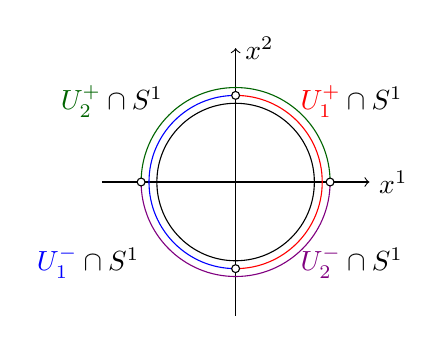
\begin{tikzpicture}
				\coordinate (U1bp) at (0,1.1);
				\coordinate (U1bm) at (0,-1.1);
				\coordinate (U2bp) at (1.2,0);
				\coordinate (U2bm) at (-1.2,0);
		
				\node[above right] at (.7,.7) {$\textcolor{red}{U_1^+} \cap S^1$};
				\node[below left] at (-1.1,-.7) {$\textcolor{blue}{U_1^-} \cap S^1$};
		
				\node[above left] at (-.8,.7) {$\textcolor{DarkGreen}{U_2^+} \cap S^1$};
				\node[below right] at (.7,-.7) {$\textcolor{violet}{U_2^-} \cap S^1$};
		
				\draw[->] (-1.7,0) -- (1.7,0) node[right]{$x^1$};
				\draw[->] (0,-1.7) -- (0,1.7) node[right]{$x^2$};
				
				\draw (0,0) circle (1);
				\draw[red] (U1bm) arc (-90:90:1.1);
				\draw[blue] (U1bp) arc (90:270:1.1);
				\draw[DarkGreen] (U2bp)  arc (0:180:1.2);
				\draw[violet] (U2bm) arc (180:360:1.2);
				\draw[fill = white] (U1bp) circle (.05);
				\draw[fill = white] (U1bm) circle (.05);
				\draw[fill = white] (U2bp) circle (.05);
				\draw[fill = white] (U2bm) circle (.05);
			\end{tikzpicture}
			\caption{$S^1$ のアトラス}
			% \label{}
		\end{subfigure}
		\hspace{5mm}
		\begin{subfigure}{0.4\columnwidth}
			\centering
			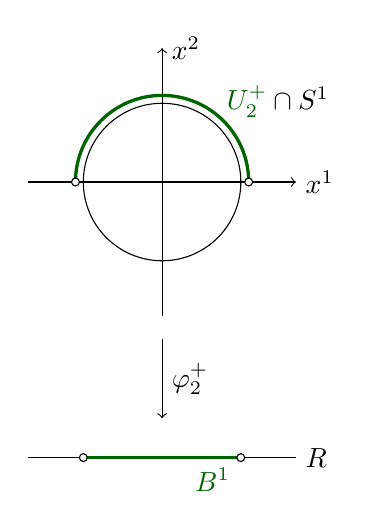
\begin{tikzpicture}
				\coordinate (U2bp) at (1.1,0);
				\coordinate (U2bm) at (-1.1,0);
		
				\draw[->] (-1.7,0) -- (1.7,0) node[right]{$x^1$};
				\draw[->] (0,-1.7) -- (0,1.7) node[right]{$x^2$};
				\draw (-1.7,-3.5) -- (1.7, -3.5) node[right]{$\mathbb{R}$};
		
				\draw[->] (0,-2) -- (0, -3);
				\node[right] at (0, -2.5) {$\varphi_2^+$};
		
				\draw[very thick, DarkGreen] (-1,-3.5) -- (1,-3.5) node[below left]{$B^1$};
				\draw (0,0) circle (1);
				\draw[very thick, DarkGreen] (U2bp)  arc (0:180:1.1);
				\node[above right] at (.7,.7) {$\textcolor{DarkGreen}{U_2^+} \cap S^1$};
				\draw[fill = white] (U2bp) circle (.05);
				\draw[fill = white] (U2bm) circle (.05);
				\draw[fill = white] (-1, -3.5) circle (.05);
				\draw[fill = white] (1, -3.5) circle (.05);
			\end{tikzpicture}
			\caption{$S^1$ のチャート $(U_2^+\cap S^1,\, \varphi_2^+)$}
			% \label{}
		\end{subfigure}
		\caption{$S^1$ の場合}
	\end{figure}%
	
	 $i = 1,\, \dots,\, n+1$ に対して,$\mathbb{R}^{n+1}$ の開集合
	\begin{align}
		U_i^+ &\coloneqq \bigl\{\, (x^1,\, \dots,\, x^{n+1}) \in \mathbb{R}^{n+1} \bigm| x^i > 0 \,\bigr\} \\
		U_i^- &\coloneqq \bigl\{\, (x^1,\, \dots,\, x^{n+1}) \in \mathbb{R}^{n+1} \bigm| x^i < 0 \,\bigr\} 
	\end{align}
	を定める.
	連続写像
	\begin{align}
		f \colon B^n \lto \mathbb{R},\; (x^1,\, \dots,\, x^n) \lmto \sqrt{1-\sum_{i=1}^n (x^i)^2}
	\end{align}
	を考える.すると $\forall (x^1,\, \dots,\, x^{n+1}) \in U_i^{\pm} \cap S^n$ は
	\begin{align}
		(x^1,\, \dots,\, \widehat{x^i},\, \dots,\, x^{n+1}) \in B^n,\; x^i = \pm f(x^1,\, \dots,\, \widehat{x^i},\, \dots,\, x^{n+1})
	\end{align}
	を充たす.ただし $\widehat{x^i}$ は第 $i$ 成分を除くことを意味する.
	つまり,$U_i^{\pm} \cap S^n$ は\hyperref[ex:graph-of-function]{関数のグラフ}
	\begin{align}
		U_i^{\pm} \cap S^n = \bigl\{\, (x^1,\, \dots,\, \widehat{x^i},\, \dots,\, x^{n+1};\, x^i) \in B^n \times \mathbb{R} \bigm| x^i = \pm f(x^1,\, \dots,\, \widehat{x^i},\, \dots,\, x^{n+1})\,\bigr\} 
	\end{align}
	である.故に第 $i$ 成分以外への射影
	\begin{align}
		\varphi_i^{\pm} \colon U_i^{\pm} \cap S^n \lto B^n,\; (x^1,\, \dots,\, x^{n+1}) \lmto \mqty(x^1 \\ \vdots \\ \widehat{x^i} \\ \vdots \\ x^{n+1})
	\end{align}
	との組 $(U^{\pm}_i,\, \varphi^{\pm}_i)$ は $n$ 次元位相多様体 $S^n$ の\hyperref[def.localcoord]{チャート}である.
	$2n+2$ 枚のチャートからなる族
	\begin{align}
		\Familyset[\big]{(U_i^+,\, \varphi_i^+),\, (U_i^-,\, \varphi_i^-)}{i=1,\, \dots,\, n+1}
	\end{align}
	は $S^n$ の\hyperref[def.atlas]{アトラス}となる.
\end{myexample}

\begin{myexample}[label=ex:topomani-projective]{$n$ 次元実射影空間}
	 $\mathbb{R}^{n+1}$ の1次元部分実ベクトル空間全体がなす集合の上に,商写像
	\begin{align}
		\pi \colon \mathbb{R}^{n+1}\setminus \{0\} \lto \mathbb{R}P^n,\; x \lmto \Span \{x\}
	\end{align}
	による\hyperref[def.quotopo]{商位相}を入れてできる位相空間を $n$ 次元\textbf{実射影空間} (real projective space) と呼び,$\bm{\mathbb{R}P^n}$ と書く.$\mathbb{R}^{n+1}$ の原点を通る直線全体がなす商位相空間と言っても良い.
	$[x] \coloneqq \pi(x) \in \mathbb{R}P^n$ と書くことにする.
	\begin{mylem}[label=lem:RP-Hausdorff]{}
		\begin{enumerate}
			\item $\mathbb{R}P^n$ はHausdorff空間である.
			\item $\mathbb{R}P^n \approx S^n / \{\pm 1\}$ である.
		\end{enumerate}
	\end{mylem}
	\begin{proof}
		\begin{enumerate}
			\item 
			$\braket{\cdot}{\cdot}$ をEuclid内積,$\abs{\cdot}$ をEuclidノルムとする.
			
			$x,\, y \in \mathbb{R}^{n+1}\setminus\{0\}$ が $[x] \neq [y]$ を充たすとする.このとき $x,\, y$ は線型独立だから $\frac{\abs{\braket{x}{y}}}{\abs{x} \abs{y}} \in [0,\, 1)$ である.よって $\frac{\abs{\braket{x}{y}}}{\abs{x} \abs{y}} < r_1 < r_2 < 1$ を充たす実数 $r_1,\, r_2$ が存在する.
			
			ここで写像
			\begin{align}
				f \colon \mathbb{R}P^n \lto [0,\, 1],\; [u] \lmto \frac{\abs{\braket{x}{u}}}{\abs{x}\abs{u}}
			\end{align}
			を考える.$[u] = [v] \in \mathbb{R}P^n$ ならばある $\lambda \in \mathbb{R}$ が存在して $u = \lambda v$ と書けるので $f([u]) = f([v])$ が言える.i.e. $f$ は $[u]$ の代表元の取り方によらず,well-definedである.
			$\pi$ が商写像でかつ $f \circ \pi$ が連続であることから $f$ も連続である.
			従って,$[0,\, 1]$ の開集合 $[0,\, r_1),\, (r_2,\, 1] \subset [0,\, 1]$ の $f$ による逆像 $U_1 \coloneqq f^{-1}\bigl([0,\, r_1)\bigr),\, U_2 \coloneqq f^{-1}\bigl((r_2,\, 1]\bigr)$ はどちらも $\mathbb{R}P^n$ の開集合で,かつ $U_1 \cap U_2 = \emptyset$ である.
			$f([y]) \in [0,\, r_1)$ かつ $f([x]) = 1 \in (r_2,\, 1]$ なので $[y] \in U_1,\, [x] \in U_2$ であり,証明が完了した.
			\item $\forall x,\, y \in S^n$ について, $[x] = [y]$ ならば $\lambda \in \mathbb{R}$ が存在して $x = \lambda y$ と書けるが,$x,\, y \in S^n$ なので $1=\abs{x} =\abs{\lambda y} = \abs{\lambda}$ でなくてはならない.故に $\lambda \in \{\pm 1\}$ である.
			i.e. $\pi$ の制限 $\pi|_{S^n} \colon S^n \lto \mathbb{R}P^n$ は2対1の連続写像である.従って商写像 $\varpi \colon S^n \lto S^{n}/\{\pm 1\},\; x \lmto \{\pm 1\}x$ が全単射連続写像 $\overline{\pi|_{S^n}} \colon S^n/\{\pm 1\} \lto \mathbb{R}P^n,\; \{\pm 1\} x \lmto [x]$ を一意的に誘導する.
			$\overline{\pi|_{S^n}}$ はコンパクト空間からHausdorff空間への連続な全単射だから同相写像である.
		\end{enumerate}
	\end{proof}
	$S^n /\{\pm 1\}$ はコンパクトなので明らかに\hyperref[def:second-countable]{第2可算}である.

	 $i = 1,\, \dots,\, n+1$ に対して,開集合 $\tilde{U_i} \subset \mathbb{R}^{n+1} \setminus \{0\}$ を
	\begin{align}
		\tilde{U_i} \coloneqq \bigl\{\, (x^1,\, \dots,\, x^{n+1}) \in \mathbb{R}^{n+1} \bigm| x^i \neq 0 \,\bigr\} 
	\end{align}
	とし,$U_i \coloneqq \pi(\tilde{U_i})$ とおく.
	このとき $\pi^{-1} \bigl( \pi(\tilde{U_i}) \bigr)$ なので制限 $\pi|_{\tilde{U_i}} \tilde{U_i} \lto U_i$ は商写像である.
	
	ここで写像
	\begin{align}
		\varphi_i \colon U_i \lto \mathbb{R}^n,\; [x^1,\, \dots,\, x^{n+1}] \lmto \mqty( \frac{x^1}{x^i} \\ \vdots \\ \frac{x^{i-1}}{x^i} \\ \frac{x^{i+1}}{x^i} \\ \vdots \\ \frac{x^{n+1}}{x^i} ) 
	\end{align}
	を考える.$\varphi_i$ は $0$ でない定数倍に関して不変なのでwell-definedである.$\pi$ が商写像で $\varphi_i \circ \pi$ が連続なので $\varphi_i$ も連続である.さらに,
	\begin{align}
		\varphi_i^{-1}\colon \mathbb{R}^n \lto U_i,\; \mqty(u^1 \\ \vdots \\ u^n) \lmto [u^1,\, \dots,\, u^{i-1},\, 1,\, u^{i+1},\, \dots,\, u^n]
	\end{align}
	が連続な\footnote{写像 $\psi_i \colon \mathbb{R}^n \lto \mathbb{R}^{n+1} \setminus \{0\},\; (u^1,\, \dots,\, u^n) \lmto (u^1,\, \dots,\, u^{i-1},\, 1,\, u^{i+1},\, \dots,\, u^n)$ は明らかに連続なので,$\varphi_i^{-1} = \pi \circ \psi_i$ は連続写像の合成となって連続である.}逆写像なので $\varphi_i$ は同相写像で,組 $(U_i,\, \varphi_i)$ は $n$ 次元\hyperref[def.topomani]{位相多様体} $\mathbb{R}P^n$ の\hyperref[def.localcoord]{チャート}である.$n+1$ 枚のチャートからなる族
	\begin{align}
		\Familyset[\big]{(U_i,\, \varphi_i)}{i = 1,\, \dots,\, n+1}
	\end{align}
	が\hyperref[def.atlas]{アトラス}となる.
\end{myexample}

\begin{myexample}[label=ex:product-mani]{積多様体}
	次元 $m,\, n$ の\hyperref[def.topomani]{位相多様体} $M,\, N$ を与える.
	このとき\hyperref[def.prodtopo]{積空間} $M \times N$ は\hyperref[def:second-countable]{第2可算}かつ\hyperref[def.separation]{Hausdorff}であ流ことが知られている.

	$\forall (p,\, q) \in M \times N$ に対して,$M,\, N$ のチャート $(U,\, \varphi),\, (V,\, \psi)$ が存在する.
	このとき写像
	\begin{align}
		\varphi \times \psi \colon U \times V \lto \mathbb{R}^{m+n},\; (x,\, y) \lmto \bigl( \varphi(x),\, \psi(y) \bigr) 
	\end{align}
	は $U \times V$ から $\mathbb{R}^{m+n}$ の開集合 $(\varphi \times \psi) (U\times V)$ への同相写像であり,組 $(U\times V,\, \varphi \times \psi)$ は $M \times N$ の
	\hyperref[def.localcoord]{チャート}を定める.

	\textbf{トーラス} $S^1 \times S^1$ は積多様体の例である.より一般に,$n$ 次元トーラスを $n$ 個の $S^1$ の積多様体として定義する.
\end{myexample}

\section{$C^\infty$ 多様体}

まず,$\mathbb{R}^n$ の微分同相を定義しておく.
\begin{mydef}[label=def.diffeomo]{($\mathbb{R}^n$ における)微分同相}
	$U,\, V$ を\underline{ $\mathbb{R}^n$ の開集合}とする.
	同相写像 $\varphi \colon U \xrightarrow{\approx} V$ が\textbf{微分同相} (diffeomorphism) であるとは,$\varphi$ とその逆写像 $\varphi^{-1}$ がともに $C^\infty$ 写像であることを言う.
\end{mydef}

\subsection{$C^\infty$ 構造}

\hyperref[def.topomani]{位相多様体} $M$ のアトラスの座標変換は同相写像であったが,そのままだと微積分との相性が悪い.
そこで,座標変換が何回でも微分可能であるような多様体を定義する.
\begin{mydef}[label=diffmani]{$C^\infty$ 多様体}
	$M$ を\hyperref[def.topomani]{位相多様体}とし,$M$ の\hyperref[def.atlas]{アトラス} $\mathcal{S} = \bigl\{\, (U_\lambda,\, \varphi_\lambda) \,\bigr\}_{\lambda \in \Lambda}$ を与える.
	\begin{itemize}
		\item $\mathcal{S}$ が\textbf{$\bm{C^\infty}$ アトラス}であるとは,$\forall \alpha,\, \beta \in \Lambda$ に対して座標変換
		\begin{align}
			f_{\beta\alpha} \colon \varphi_\alpha(U_\alpha\cap U_\beta) \xrightarrow{\approx} \varphi_\beta (U_\alpha\cap U_\beta)
		\end{align}
		が\hyperref[def.diffeomo]{微分同相}であること.
		\item $\mathcal{S}$ が\textbf{$\bm{C^\infty}$ アトラス}であるとき,$\mathcal{S}$ は $M$ 上の\textbf{$\bm{C^\infty}$ 構造}を定めるという.
		\item $C^\infty$ 構造の与えられた多様体のことを\textbf{$\bm{C^\infty}$ 多様体}と呼ぶ.
	\end{itemize}
\end{mydef}

\begin{marker}
	文献によっては $C^\infty$ 多様体のことを指して\textbf{滑らかな多様体} (smooth manifold) とか,\textbf{可微分多様体},\textbf{微分可能多様体} (differentiable manifold) と呼んでいることがあるので注意.この資料では以降一貫して $C^\infty$ 多様体と言うことにする.
\end{marker}

座標変換 $f_{\beta\alpha}$ の定義域と終域は $\mathbb{R}^n$ の開集合なので,\hyperref[def.diffeomo]{ $\mathbb{R}^n$ における微分同相の定義}で十分なのである.
なお,与えられた写像 $f \colon \mathbb{R}^n \lto \mathbb{R}^n$ が微分同相であるかどうかを判定する問題は,一般には容易でない.
技術的には,例えば逆函数定理などが有用である:
\begin{mytheo}[label=thm.inverse]{逆函数定理}
	$U$ を$\mathbb{R}^n$ の開集合とし,$C^\infty$ 写像 $\varphi \colon U \to \mathbb{R}^n$ を与える.
	ある1点 $x \in U$ における $\varphi$ のJacobianが $0$ でなければ,$x$ のある\hyperref[def:neighborhood]{開近傍} $x \in V \subset U$ が存在して $\varphi(V) \subset \mathbb{R}$ は $\mathbb{R}^n$ の開集合となり,
	$\varphi$ の制限
	\begin{align}
		\varphi|_V \colon V \lto \varphi(V)
	\end{align}
	は\hyperref[def.diffeomo]{微分同相}になる.
\end{mytheo}

\begin{proof}
	例えば~\cite[Theorem C.34]{Lee12}を参照.
\end{proof}

\begin{myexample}[]{$\mathbb{R}^3$ のチャート}
	 \hyperref[def.topomani]{位相多様体} $\mathbb{R}^3$ の最も簡単な\hyperref[def.localcoord]{チャート}は
	\begin{itemize}
		\item $U_1 \coloneqq \mathbb{R}^3$ を点 $p$ の\hyperref[def.localcoord]{座標近傍}とする.
		\item 同相写像\footnote{ややこしいようだが,左辺は位相多様体 $\mathbb{R}^3$ の点としての $(x,\, y,\, z)$ で,右辺は\hyperref[def.localcoord]{チャート}の定義としての $\mqty(x \\ y \\ z)$ である.実際のところは $\varphi_1 = \mathrm{id}_{\mathbb{R}^3}$ である.}
		\begin{align}
			\varphi_1 \colon U_1 \lto \mathbb{R}^3,\;
			(x,\, y,\, z) \lmto \mqty(x^1(x,\, y,\, z) \\ x^2(x,\, y,\, z) \\ x^3(x,\, y,\, z)) = \mqty(x \\ y \\ z)
		\end{align}
	\end{itemize}
	の組 $(U_1,\, \varphi_1)$ で,チャートを1枚だけ含む族
	\begin{align}
		\mathcal{A}_1 \coloneqq \bigl\{(U_1,\, \varphi_1)\bigr\}
	\end{align}
	が $\mathbb{R}^3$ の\hyperref[def.atlas]{$C^\infty$ アトラス}になる.
	
	 一方で,$\mathbb{R}^3$ の\hyperref[def.openset]{開集合}
	\begin{align}
		U_2 &\coloneqq \bigl\{\, (x,\, y,\, z) \in \mathbb{R}^3 \bigm| x > 0,\, z > 0 \,\bigr\} = (0,\, \infty) \times \mathbb{R} \times (0,\, \infty), \\
	\end{align}
	の上で定義される連続写像
	\begin{align}
		\varphi_2 \colon U_2 \lto \varphi_2(U_2),\;
		(x,\, y,\, z) \lmto \mqty(r(x,\, y,\, z) \\ \theta(x,\, y,\, z) \\ \phi(x,\, y,\, z)) = \mqty(\sqrt{x^2 + y^2 + z^2} \\ \arctan(y/z) \\ \arctan(y/x))
	\end{align}
	を考える.
	$\varphi_2 (U_2) = (0,\, \infty) \times (0,\, \pi/2) \times (-\pi/2,\, \pi/2)$ であり,
	逆写像
	\begin{align}
		\varphi_2^{-1} \colon \varphi_2(U_2) \lto U_2,\;
		\mqty(r \\ \theta \\ \phi) \lmto (r \sin\theta \cos\phi, \, r\sin\theta \sin\phi,\, r\cos\theta)
	\end{align}
	も連続なので $\varphi_2$ は同相写像である.
	従って組 $(U_2,\, \varphi_2)$ も\hyperref[def.localcoord]{チャート}と見做せる.このチャートは\textbf{3次元極座標系}と呼ばれるものである.
	\begin{align}
		\mathbb{R}^3 = U_1 \cup U_2
	\end{align}
	なので,チャートの族
	\begin{align}
		\mathcal{A}_2 \coloneqq \bigl\{(U_1,\, \varphi_1),\, (U_2,\, \varphi_2)  \bigr\}
	\end{align}
	もまた位相多様体 $\mathbb{R}^3$ の\hyperref[def.atlas]{アトラス}になる.
	アトラス $\mathcal{A}_2$ におけるチャートの重なりは
	\begin{align}
		U_1 \cap U_2 = U_2
	\end{align}
	で,この間の座標変換は
	\begin{align}
		\varphi_1 \circ \varphi_2^{-1} \colon \varphi_2(U_2) &\lto \varphi_1(U_2) \\
		\mqty(r \\ \theta \\ \phi) &\lmto \mqty(x^1(r,\, \theta,\, \phi) \\ x^2(r,\, \theta,\, \phi) \\ x^3(r,\, \theta,\, \phi)) = \mqty(r \sin\theta \cos\phi \\ r\sin\theta \sin\phi \\ r\cos\theta)
	\end{align}
	となる.$\varphi_1 \circ \varphi_2^{-1}$ のJacobianは
	\begin{align}
		\mqty|\pdv{x^1}{r} & \pdv{x^1}{\theta} & \pdv{x^1}{\phi} \\ \pdv{x^2}{r} & \pdv{x^2}{\theta} & \pdv{x^3}{\phi} \\ \pdv{x^3}{r} & \pdv{x^3}{\theta} & \pdv{x^3}{\phi}| = r^2 \sin \theta
	\end{align}
	で $U_2$ 上の全ての点で正だから,\hyperref[thm.inverse]{逆関数定理}により $\varphi_1 \circ \varphi_2^{-1}$ が\hyperref[def.diffeomo]{微分同相写像}であるとわかる.
	つまり,アトラス $\mathcal{A}_2$ は\hyperref[diffmani]{$C^\infty$ アトラス}であり,$\mathbb{R}^3$ の $C^\infty$ 構造の\underline{1つ}を定める.

	 他には $\mathbb{R}^3$ の開集合
	\begin{align}
		U_3 \coloneqq \bigl\{\, (x,\, y,\, z) \in \mathbb{R}^3 \bigm| x > 0 \,\bigr\}  = (0,\, \infty) \times \mathbb{R}^2
	\end{align}
	の上で定義される同相写像
	\begin{align}
		\varphi_3 \colon U_3 \lto \varphi_3(U_3),\;
		(x,\, y,\, z) \lmto \mqty(\rho(x,\, y,\, z) \\ \phi(x,\, y,\, z) \\ z(x,\, y,\, z)) = \mqty(\sqrt{x^2 + y^2 + z^2} \\ \arctan(y/x) \\ z)
	\end{align}
	を考えることもできる.
	$\varphi_3(U_3) = (0,\, \infty) \times (-\pi/2,\, \pi/2) \times \mathbb{R}$ で,
	逆写像は
	\begin{align}
		\varphi_3^{-1} \colon \varphi_3 (U_3) \lto U_3,\;
		\mqty(\rho \\  \phi \\ z) \lmto (\rho \cos \phi,\, \rho \sin \phi,\, z)
	\end{align}
	である.チャート $(U_3,\, \varphi_3)$ は\textbf{円筒座標系}として知られる.
	チャートの族
	\begin{align}
		\mathcal{A}_3 \coloneqq \bigl\{(U_1,\, \varphi_1),\, (U_3,\, \varphi_3)  \bigr\}
	\end{align}
	は位相多様体 $\mathbb{R}^3$ のアトラスを成す.$\mathcal{A}_3$ におけるチャートの重なりは
	\begin{align}
		U_1 \cap U_3 = U_3
	\end{align}
	で,座標変換は
	\begin{align}
		\varphi_1 \circ \varphi_3^{-1} \colon \varphi_3(U_3) \lto \varphi_1(U_3), \;
		\mqty(\rho \\  \phi \\ z) \lmto \mqty(x^1(\rho,\, \phi,\, z) \\ x^2(\rho,\, \phi,\, z) \\ x^3(\rho,\, \phi,\, z)) =  \mqty(\rho \cos\phi \\ \rho \sin \phi \\ z)
	\end{align}
	となる.$\varphi_1 \circ \varphi_3^{-1}$ のJacobianは $\rho$ であるから $\varphi_3(U_3)$ の全ての点において正であり,\hyperref[thm.inverse]{逆関数定理}から\hyperref[def.diffeomo]{微分同相写像}であるとわかる.
	つまり,アトラス $\mathcal{A}_3$ もまた\hyperref[diffmani]{$C^\infty$ アトラス}であり,$\mathbb{R}^3$ の上に \underline{$\mathcal{A}_2$ とは別の $C^\infty$ 構造を定める.}
\end{myexample}

この例からも,$C^\infty$ アトラスが複数存在し得ることがわかる.
しかし,明かに $\mathcal{A}_2 \cup \mathcal{A}_3$ もまた $C^\infty$ アトラスになるので,$\mathcal{A}_2$ が定める $C^\infty$ 構造と $\mathcal{A}_3$ が定める $C^\infty$ 構造を区別するのは話を無駄にややこしくしているように思われる.
そこで,考えられる限り最大の $C^\infty$ アトラスを構成できると便利である.

\begin{mydef}[label=manieq]{$C^\infty$ アトラスの同値関係}
	\hyperref[diffmani]{$C^\infty$ 多様体} $M$ 上の $C^\infty$ アトラス全体の集まりを $\mathscr{A}$ と書く.
	$\mathscr{A}$ 上の同値関係 $\sim$ を以下のように定める:
	\begin{align}
		\sim\; \coloneqq \{(\mathcal{S},\, \mathcal{T}) \in \mathscr{A} \times \mathscr{A} \mid \mathcal{S} \cup \mathcal{T} \in \mathscr{A} \}
	\end{align}
	$\mathcal{S} \sim \mathcal{T}$ のとき,$\mathcal{S},\, \mathcal{T}$ は\textbf{両立する}と言う.
\end{mydef}

% \begin{proof}
% 	定義\ref{def:topomani-compatible}のときと全く同様に示すことができる.
% \end{proof}

\begin{proof}
	同値関係の公理\ref{ax.equiv}を充していることを示す.
	\begin{enumerate}
		\item $\mathcal{S} \cup \mathcal{S} = \mathcal{S}$ より反射律を充たす.
		\item $\mathcal{S} \cup \mathcal{T} = \mathcal{T} \cup \mathcal{S}$ より対称律を充たす.
		\item 任意のチャート $(S,\, \varphi) \in \mathcal{S},\; (U,\, \psi) \in \mathcal{U}$ をとる.$\mathcal{S} \sim \mathcal{T}$ かつ $\mathcal{T} \sim \mathcal{U}$ のとき,$\varphi(S \cap U),\, \psi(S \cap U)$ が $\mathbb{R}^n$ の開集合でかつ $\psi \circ \varphi^{-1} \colon \varphi(S \cap U) \to \psi(S \cap U)$ が\hyperref[def.diffeomo]{微分同相}であることを示せばよい.
		
		 仮定よりそれぞれのチャートは $\forall (T_\lambda,\, \phi_\lambda) \in \mathcal{T}$ と両立するので,$\phi_\lambda(S \cap T_\lambda),\, \phi_\lambda (U \cap T_\lambda) \subset \mathbb{R}^n$ は開集合である.
		$\phi_\lambda$ は同相写像なので全単射であり,従って補題\ref{lem:sets}-(9)より
		\begin{align}
			\phi_\lambda(S \cap T_\lambda) \cap \phi_\lambda (U \cap T_\lambda) = \phi_\lambda (S \cap U \cap T_\lambda) 
		\end{align}
		が成り立つから, $\phi_\lambda(S \cap T_\lambda) \cap \phi_\lambda (U \cap T_\lambda) $ は $\mathbb{R}^n$ の開集合である.
		$\varphi \circ \phi_\lambda^{-1}$ は同相写像であるから
		\begin{align}
			\varphi(S \cap U \cap T_\lambda) = (\varphi \circ \phi_\lambda^{-1})(\phi_\lambda (S \cap U \cap T_\lambda))
		\end{align}
		も $\mathbb{R}^n$ の開集合である.ここで補題\ref{lem:sets}-(1)を使うと\footnote{選択公理を認める.},
		\begin{align}
			\varphi(S \cap U) = \varphi(S \cap U \cap M) =  \varphi \left(S \cap U \cap \left(\bigcup_\lambda T_\lambda\right)\right) = \varphi \left(\bigcup_\lambda S \cap U \cap T_\lambda\right) = \bigcup_\lambda \varphi(S \cap U \cap T_\lambda)
		\end{align}
		も $\mathbb{R}^n$ の開集合であると分かる.全く同様の議論により $\psi (S \cap U)$ も $\mathbb{R}^n$ の開集合.

		 次に,$\psi \circ \varphi^{-1} \colon \varphi (S \cap U) \to \psi (S \cap U)$ が微分同相であることを示す.仮定より任意のチャート $(T_\lambda,\, \phi_\lambda) \in \mathcal{T}$ に対して
		$\phi_\lambda \circ \varphi^{-1} \colon \varphi (S \cap T_\lambda) \to \phi_\lambda (S \cap T_\lambda)$ は微分同相.従ってこれの $\varphi(S \cap U \cap T_\lambda)$ への制限
		\begin{align}
			\eval{\phi_\lambda \circ \varphi^{-1}}_{\varphi(S \cap U \cap T_\lambda)} \colon  \varphi (S \cap U \cap T_\lambda) \to \phi_\lambda (S \cap U \cap T_\lambda)
		\end{align}
		もまた微分同相である.$\eval{\psi \circ \phi^{-1}_\lambda}_{\phi_\lambda(S \cap U \cap T_\lambda)}$ に関しても同様なので,これらの合成
		\begin{align}
			\psi \circ \varphi^{-1} \colon \varphi (S \cap U \cap T_\lambda) \to \psi (S \cap U \cap T_\lambda)
		\end{align}
		もまた微分同相.ここで $\varphi,\, \psi$ が全単射であること,および $M = \bigcup_{\lambda} T_\lambda$ を使うと
		\begin{align}
			\varphi(S \cap U) = \bigcup_\lambda \varphi(S \cap U \cap T_\lambda),\quad \psi(S \cap U) = \bigcup_\lambda \psi(S \cap U \cap T_\lambda)
		\end{align}
		が分かるので,
		\begin{align}
			\psi \circ \varphi^{-1} \colon \varphi(S \cap U) \to \psi(S \cap U)
		\end{align}
		も微分同相写像である.
	\end{enumerate}
\end{proof}

\begin{mydef}[label=maxatlas]{微分構造・極大アトラス}
	\hyperref[diffmani]{$C^\infty$ 多様体} $M$ の $C^\infty$ アトラス $\mathcal{S}$ を与える.
	\begin{itemize}
		\item 定義\ref{manieq}で定めた同値関係による $\mathcal{S}$ の同値類 $[\mathcal{S}] \subset \mathscr{A}$ を $M$ の\textbf{微分構造} (differential structure) と呼ぶ.
		\item $C^\infty$ アトラス $\mathcal{S}$ の\textbf{極大アトラス} (maximal atlas) $\mathcal{S}^+$ を以下のように定義する:
		\begin{align}
			\mathcal{S}^+ \coloneqq \bigcup_{\mathcal{T} \in [\mathcal{S}]} \mathcal{T}.
		\end{align}
	\end{itemize}
\end{mydef}

\begin{marker}
	実は,極大アトラスは1通りとは限らないことが知られている.しかし,本資料内ではあまり気にしなくても良い.
\end{marker}

以降では,断らない限り多様体のアトラスは全て極大アトラスであるとする.

\begin{myexample}[label=ex:diffmani-n-sphere]{$S^n$ の微分構造}
	\exref{ex:topomani-n-sphere}で構成した\hyperref[def.atlas]{アトラス}
	\begin{align}
		\mathcal{A}_{S^n} \coloneqq \Familyset[\big]{(U_i^{\pm},\, \varphi_i^{\pm})}{i=1,\, \dots,\, n+1}
	\end{align}
	の座標変換を顕に書くと,$i > j$ のとき
	\begin{align}
		\varphi_i^{\pm} \circ (\varphi_j^{\textcolor{red}{\pm}})^{-1} \colon \mqty(u^1 \\ \vdots \\ u^n) \lmto \mqty(u^1 \\ \vdots \\ \widehat{u^i} \\ \vdots \\ \underbrace{\textcolor{red}{\pm} \sqrt{1- \abs{\bm{u}}^2}}_{j} \\ \vdots \\ u^n)
	\end{align}
	で,$i=j$ のとき $\varphi_i^{\pm} \circ (\varphi_j^{\pm})^{-1} = \mathrm{id}_{B^n}$ であり,\hyperref[def.diffeomo]{微分同相写像}である.
	従って $\mathcal{A}_{S^n}$ は\hyperref[diffmani]{$C^\infty$ アトラス}で,これの\hyperref[maxatlas]{極大アトラス}を $S^n$ の標準的な\hyperref[maxatlas]{微分構造}とする.
\end{myexample}

\begin{myexample}[label=ex:stereographic-projection]{立体射影}
	$S^n$ の上に\exref{ex:diffmani-n-sphere}の $\mathcal{A}_{S^n}$ とは異なる\hyperref[diffmani]{$C^\infty$ アトラス}を構成する.この方法は\textbf{立体射影} (stereographic projection) として知られる.
	\begin{figure}[H] 
		\centering
		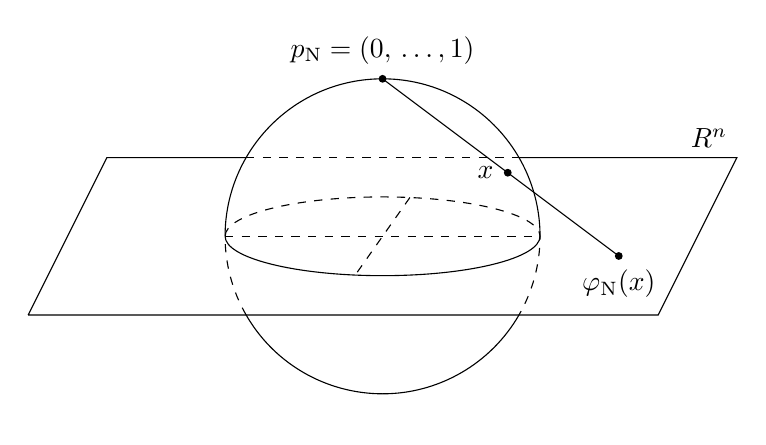
\begin{tikzpicture} 
			\coordinate (A) at (3,-0.25);
			\coordinate (P) at (0,2);

			\draw (0:2cm)   arc[radius=2cm,start angle=0,end angle=180]
				  (210:2cm) arc[radius=2cm,start angle=210,end angle=330];
			\draw (180:2cm) arc[x radius=2cm, y radius=0.5cm, start angle=180,end angle=360];

			\draw [dashed] (210:2cm) 
				  arc[start angle=210,delta angle=-30,radius=2cm]
				  arc[start angle=180,delta angle=-180,x radius=2cm,y radius=0.5cm]
				  arc[start angle=0,delta angle=-30,radius=2cm];

			\draw [dashed] (80:2cm and 0.5cm) -- (260:2cm and 0.5cm);
			\draw [dashed] (150:2cm) coordinate(ul) -- (30:2cm) coordinate(ur);

			\draw (-4.5,-1) -- (3.5,-1) -- (4.5,1) node[anchor=south east] {$ \mathbb{R}^n $} -- (ur) (ul) -- (-3.5,1) -- (-4.5,-1);

			\draw (A) -- (P) coordinate[pos=0.47](B);
			\path (A) node[circle, fill, inner sep=1pt, label=below:{$ \varphi_{\mathrm{N}}(x) $}]{};
			\path (B) node[circle, fill, inner sep=1pt, label=left:{$x$}]{};
			\path (P) node[circle, fill, inner sep=1pt, label=above:{$ p_{\mathrm{N}} = (0,\, \dots ,1) $}]{};
			\draw [dashed] (-2,0) -- (2,0);
		\end{tikzpicture}
		\caption{立体射影}
	\end{figure}
	
	 $S^n$ の「北極点」を $p_{\mathrm{N}} = (0,\, \dots ,\, 0,\,  1) \in \mathbb{R}^{n+1}$ とおく.$U_{\mathrm{N}} \coloneqq S^n \setminus \{ p_{\mathrm{N}} \}$ は $S^n$ の開集合である.
	点 $x = (x^1,\, \dots,\, x^{n+1}) \in U_{\mathrm{N}}$ を任意にとる.
	$p_{\mathrm{N}}$ と $x$ を通る $\mathbb{R}^{n+1}$ の直線は
	$\Familyset[\big]{t x + (1-t) p_{\mathrm{N}}}{t \in \mathbb{R}}$
	と書けるので,この直線と超平面 $x^{n+1} = 0$ の交点は,$t$ の方程式 $t x^{n+1} + (1-t) = 0$ を解くことで
	\begin{align}
		\frac{1}{1-x^{n+1}} x + \left( 1 - \frac{1}{1-x^{n+1}} \right) p_{\mathrm{N}} = \left( \frac{x^1}{1-x^{n+1}},\, \dots,\, \frac{x^n}{1-x^{n+1}},\, 0 \right) \in \mathbb{R}^n \times \{0\}
	\end{align}
	のただ1つであることがわかる.以上の考察から同相写像
	\begin{align}
		\varphi_{\mathrm{N}} \colon U_{\mathrm{N}} \lto \mathbb{R}^{n},\; (x^1,\, \dots,\, x^{n+1}) \lmto \mqty(x_{\mathrm{N}}{}^1(x^1,\, \dots,\, x^{n+1}) \\ \vdots \\ x_{\mathrm{N}}{}^n(x^1,\, \dots,\, x^{n+1})) = \mqty(\frac{x^1}{1-x^{n+1}}\\ \vdots \\ \frac{x^n}{1-x^{n+1}})
	\end{align}
	が得られる.逆写像を顕に書くと
	\begin{align}
		\varphi_{\mathrm{N}}^{-1} \colon \mathbb{R}^n \lto S^n,\;
		\mqty(x_{\mathrm{N}}{}^1 \\ \vdots \\ x_{\mathrm{N}}{}^n) \lmto \left(\frac{2 x_{\mathrm{N}}{}^1}{\abs{\vb*{x}_{\mathrm{N}}}^2 +1}, \, \dots,\, \frac{2 x_{\mathrm{N}}{}^n}{\abs{\vb*{x}_{\mathrm{N}}}^2 +1},\, \frac{\abs{\vb*{x}_{\mathrm{N}}}^2 -1}{\abs{\vb*{x}_{\mathrm{N}}}^2 +1}\right)
	\end{align}
	となる.組 $(U_{\mathrm{N}},\, \varphi_{\mathrm{N}}) = \chart{U_{\mathrm{N}}}{x_{\mathrm{N}}{}^\mu}$ は\hyperref[def.topomani]{位相多様体} $S^n$ の\hyperref[def.topomani]{チャート}になる.
	
	 $S^n$ の「南極点」を $p_{\mathrm{S}} = (0,\, \dots ,\, 0,\,  -1)$ とおき,$S^n$ の開集合 $U_{\mathrm{S}} \coloneqq S^n \setminus \{ p_{\mathrm{S}} \}$ の上で同様の議論を行うことで
	同相写像
	\begin{align}
		\varphi_{\mathrm{S}} \colon U_{\mathrm{S}} &\lto \mathbb{R}^n,\;
		(x^1,\, \dots,\, x^{n+1}) \lmto \mqty(x_{\mathrm{S}}{}^1(x^1,\, \dots,\, x^{n+1}) \\ \vdots \\ x_{\mathrm{S}}{}^n(x^1,\, \dots,\, x^{n+1})) = \mqty(\frac{x^1}{1+x^{n+1}} \\ \vdots \\ \frac{x^n}{1+x^{n+1}}) \\
		\varphi_{\mathrm{N}}^{-1} \colon \mathbb{R}^n &\lto S^n,\;
		\mqty(x_{\mathrm{S}}{}^1 \\ \vdots \\ x_{\mathrm{S}}{}^n) \lmto \left(\frac{2 x_{\mathrm{S}}{}^1}{\abs{\vb*{x}_{\mathrm{S}}}^2 +1}, \, \dots,\, \frac{2 x_{\mathrm{S}}{}^n}{\abs{\vb*{x}_{\mathrm{S}}}^2 +1},\, -\frac{\abs{\vb*{x}}^2 -1}{\abs{\vb*{x}}^2 +1}\right)
	\end{align}
	が得られ,組 $(U_{\mathrm{S}},\, \varphi_{\mathrm{S}}) = \chart{U_{\mathrm{S}}}{x_{\mathrm{S}}{}^\mu}$ も位相多様体 $S^n$ のチャートになる.さらに
	\begin{align}
		S^n = U_{\mathrm{N}} \cup U_{\mathrm{S}}
	\end{align}
	が成り立つので,2つのチャートを含む族
	\begin{align}
		\mathcal{A}_{\mathrm{NS}} \coloneqq \bigl\{ (U_{\mathrm{N}},\, \varphi_{\mathrm{N}}),\, (U_{\mathrm{S}},\, \varphi_{\mathrm{S}})\bigr\}
	\end{align}
	は $S^n$ の\hyperref[def.atlas]{アトラス}である.チャートの重なりは
	$U_{\mathrm{N}} \cap U_{\mathrm{S}} = S^n \setminus \{p_{\mathrm{N}},\, p_{\mathrm{S}}\}$
	なので $\varphi_{\mathrm{N}}(U_{\mathrm{N}} \cap U_{\mathrm{S}}) = \varphi_{\mathrm{S}}(U_{\mathrm{N}}\cap U_{\mathrm{S}}) = \mathbb{R}^n\setminus \{\vb*{0}\}$ であり,
	座標変換は
	\begin{align}
		\label{ex.stereo}
		\varphi_{\mathrm{S}} \circ \varphi_{\mathrm{N}}^{-1} \colon \varphi_{\mathrm{N}}(U_{\mathrm{N}} \cap U_{\mathrm{S}}) &\lto \varphi_{\mathrm{S}}(U_{\mathrm{N}}\cap U_{\mathrm{S}}),\;
		\mqty(x_{\mathrm{N}}{}^1 \\ \vdots \\ x_{\mathrm{N}}{}^n) \lmto \mqty(x_{\mathrm{N}}{}^1/\abs{\vb*{x}_{\mathrm{N}}}^2 \\ \vdots \\ x_{\mathrm{N}}{}^n/\abs{\vb*{x}_{\mathrm{N}}}^2)
	\end{align}
	で,\cinfty 級である.$\varphi_{\mathrm{N}} \circ \varphi_{\mathrm{S}}^{-1}$ も同様に\cinfty 級なので座標変換が\hyperref[def.diffeomo]{微分同相写像}であり,
	アトラス $\mathcal{A}_{\mathrm{NS}}$ は $S^n$ 上の\hyperref[diffmani]{\cinfty アトラス}である.

	$\mathcal{A}_{\mathrm{NS}}$ が\exref{ex:diffmani-n-sphere}の $C^\infty$ アトラス $\mathcal{A}_{S^n}$ と\hyperref[manieq]{両立する}ことを確認する.
	% $\irm{p}{N} \in U_{n+1}^+,\; \irm{p}{S} \in U_{n+1}^-$ で,残りの $i = 1,\, \dots,\, n$ に対しては $\{\irm{p}{N},\, \irm{p}{S}\} \not\subset U_i^{\pm}$ であることに注意する.
	まず $U_{n+1}^{\pm} \cap \irm{U}{N}$ の上の座標変換は
	\begin{align}
		\varphi_{n+1}^{\pm} \circ \varphi_{\mathrm{N}}^{-1} \colon \mqty(x_{\mathrm{N}}{}^1 \\ \vdots \\ x_{\mathrm{N}}{}^n) &\lmto \mqty(\frac{2 x_{\mathrm{N}}{}^1}{\abs{\vb*{x}_{\mathrm{N}}}^2 +1} \\ \vdots \\ \frac{2 x_{\mathrm{N}}{}^n}{\abs{\vb*{x}_{\mathrm{N}}}^2 +1}) \\
		\varphi_{\mathrm{N}} \circ (\varphi_{n+1}^{\pm})^{-1} \colon \mqty(u^1 \\ \vdots \\ u^n) &\lmto \mqty(\frac{u^1}{1\mp\sqrt{1-\abs{\bm{u}}^2}} \\ \vdots \\ \frac{u^n}{1\mp\sqrt{1-\abs{\bm{u}}^2}})
	\end{align}
	なので\hyperref[def.diffeomo]{微分同相}写像である.
	
	次に $i = 1,\, \dots,\, n$ に対しては $\{\irm{p}{N},\, \irm{p}{S}\} \not\subset U_i^{\pm} \cap \irm{U}{N}$ なので,座標変換は
	\begin{align}
		\varphi_{i}^+ \circ \varphi_{\mathrm{N}}^{-1} \colon \mqty(x_{\mathrm{N}}{}^1 \\ \vdots \\ x_{\mathrm{N}}{}^n) &\lmto \mqty(\frac{2 x_{\mathrm{N}}{}^1}{\abs{\vb*{x}_{\mathrm{N}}}^2 +1} \\ \vdots \\ \frac{2 \widehat{x_{\mathrm{N}}{}^i}}{\abs{\vb*{x}_{\mathrm{N}}}^2 +1} \\ \vdots \\ \frac{2 x_{\mathrm{N}}{}^n}{\abs{\vb*{x}_{\mathrm{N}}}^2 +1}) \\
		\varphi_{\mathrm{N}} \circ (\varphi_{i}^{\pm})^{-1} \colon \mqty(u^1 \\ \vdots \\ u^n) &\lmto \mqty(\frac{u^1}{1-u^n} \\ \vdots \\ \underbrace{\pm\frac{\sqrt{1-\abs{\bm{u}}^2}}{1-u^n}}_i \\ \vdots \\ \frac{u^{n-1}}{1-u^n})
	\end{align}
	で,\hyperref[def.diffeomo]{微分同相}写像である.$\varphi_{\mathrm{S}}$ に関しても同様に,座標変換が微分同相写像であることを直接確認できる.
	従って $\mathcal{A}_{\mathrm{NS}}$ は $\mathcal{A}_{S^n}$ と同じ\hyperref[maxatlas]{極大アトラス}に属し,$S^n$ に同じ\hyperref[maxatlas]{微分構造}を定める.
\end{myexample}

\begin{myexample}[label=ex:diffmani-finvec]{有限次元位相ベクトル空間}
	$V$ を $n < \infty$ 次元ベクトル空間とする.$V$ 上の任意のノルムによって $V$ を\hyperref[def.metric-space]{距離空間}と見做し,\hyperref[thm.metrictopo]{距離空間の標準的な位相}を入れて位相空間にする.
	% $V \cong \mathbb{R}^n$ なので,$V$ は $n$ 次元\hyperref[def.topomani]{位相多様体}になる.
	% $V$ 上の自然な\hyperref[diffmani]{$C^\infty$ 構造}は次のようにして定まる:
	$V$ の任意の基底 $\{e_1,\, \dots,\, e_n\}$ を1つとってベクトル空間の同型写像
	\begin{align}
		e \colon \mathbb{R}^n \lto V,\; (x^1,\, \dots,\, x^n) \lmto x^\mu e_\mu
	\end{align}
	を考えると,$e$ は\hyperref[def.homeo]{同相写像}でもある.従って組 $(V,\, e^{-1}) = \chart{V}{x^\mu}$ は\hyperref[def.topomani]{位相多様体} $V$ の\hyperref[def.localcoord]{チャート}になる.
	この位相多様体 $V$ の上の自然な\hyperref[diffmani]{$C^\infty$ 構造}は次のようにして定まる:
	
	別の基底 $\{e'{}_1,\, \dots,\, e'{}_n\}$ による同相写像
	\begin{align}
		e' \colon \mathbb{R}^n \lto V,\; (x'{}^1,\, \dots,\, x'{}^n) \lmto x'{}^\mu e'{}_\mu
	\end{align}
	が定めるチャート $(V,\, e'{}^{-1}) = \chart{V}{x'{}^\mu}$ を考える.基底の取り替えを表す正則行列 $[T^\mu{}_\nu]$ が存在して
	\begin{align}
		e_\mu = e'{}_{\nu}T^{\nu}{}_{\mu}
	\end{align}
	と書けるので,$\chart{V}{x^\mu}$ から $\chart{V}{x'{}^\mu}$ への座標変換は
	\begin{align}
		x'{}^\mu (x^1,\, \dots ,\, x^n) = T^{\mu}{}_\nu x^\nu\quad (\mu = 1,\, \dots,\, n)
	\end{align}
	という\hyperref[def.diffeomo]{微分同相写像}になる.i.e. チャート $\chart{V}{x^\mu},\, \chart{V}{x'{}^\mu}$ は\hyperref[manieq]{両立する}.
	アトラス $\{\chart{V}{x^\mu}\}$ の\hyperref[maxatlas]{極大アトラス}を $V$ の標準的な微分構造として定める.
\end{myexample}

\begin{myexample}[label=ex:diffmani-finmat]{行列空間}
	$m \times n$ 実行列全体の集合を $\bm{\Mat{m \times n}{\mathbb{R}}}$ と書く.$\Mat{m \times n}{\mathbb{R}}$ は行列の和と実数倍に関して $mn$ 次元ベクトル空間をなすので,\exref{ex:diffmani-finvec}によって\hyperref[diffmani]{$C^\infty$ 多様体}になる.
	特に,同相写像
	\begin{align}
		\Mat{m \times n}{\mathbb{R}} &\lto \mathbb{R}^{mn},\\ 
		\mqty[x^1{}_1 &x^1{}_2& \cdots &x^1{}_n \\ x^2{}_1 &x^2{}_2 &\cdots &x^2{}_n \\ &\vdots & \vdots &\ddots &\vdots \\ x^m{}_1 &x^m{}_2 &\cdots &x^m{}_n] &\lmto \mqty(x^1{}_1 \\ \vdots \\ x^1{}_n \\ x^2{}_1\\ \vdots \\ x^m{}_n )
	\end{align}
	などによってしばしば $\mathbb{R}^{mn}$ と同一視される.
	
	同様に,$m \times n$ 複素行列全体の集合を $\Mat{m \times n}{\mathbb{C}}$ と書くとこれは $2mn$ 次元\underline{実} \hyperref[diffmani]{$C^\infty$ 多様体}になる.

	なお,以降では行列のサイズが $n \times n$ の場合に限って $\bm{\Mat{n}{\mathbb{R}}},\, \bm{\Mat{n}{\mathbb{C}}}$ と略記する.
\end{myexample}

\begin{myexample}[label=ex:open-submani]{開部分多様体}
	$U \subset \mathbb{R}^n$ を $\mathbb{R}^n$ の開集合とする.このとき $U$ は $n$ 次元\hyperref[def.topomani]{位相多様体}であり,1枚のみのチャートを持つ\hyperref[def.atlas]{アトラス} $\{(U,\, \mathrm{id}_U)\}$ が $U$ 上の\hyperref[diffmani]{\cinfty 構造}を定める.

	より一般に,$M$ を\hyperref[diffmani]{\cinfty 多様体},$\mathcal{A}_M$ を $M$ の\hyperref[diffmani]{\cinfty アトラス}とし,$U\subset M$ を $M$ の開集合とする.
	このとき,
	\begin{align}
		\mathcal{A}_U \coloneqq \bigl\{\, (V,\, \psi) \in \mathcal{A}_M \bigm| V \subset U \,\bigr\} 
	\end{align}
	は $U$ の\hyperref[def.atlas]{\cinfty アトラス}になる.
	このようにして $M$ の開集合に\hyperref[diffmani]{\cinfty 構造}を入れてできる\hyperref[diffmani]{\cinfty 多様体}のことを\textbf{開部分多様体} (open submanifold) と呼ぶ.
\end{myexample}

\begin{myexample}[label=ex:product-diffmani]{\cinfty 積多様体}
	$M,\, N$ を\hyperref[diffmani]{\cinfty 多様体}とする.
	\exref{ex:product-mani}による積多様体 $M \times N$ のチャートは $(U_1 \times U_2,\, \varphi_1 \times \varphi_2)$ の形をしているが,任意の座標変換
	\begin{align}
		(\varphi_1 \times \varphi_2) \circ (\psi_1 \times \psi_2)^{-1} = (\varphi_1 \circ \psi_1^{-1}) \times (\varphi_2 \circ \psi_2^{-1})
	\end{align}
	は\cinfty 級なので $M \times N$ は\hyperref[diffmani]{\cinfty 多様体}でもある.
\end{myexample}


% \begin{description}
% 	\item[\textbf{立体射影}] 
% 	\item[\textbf{Riemann球面}] 
	
% 	 前述の立体射影のうち $n=2$ の場合を考え,$\mathbb{R}^2$ と $\mathbb{C}$ を微分同相写像 $(x,\, y) \mapsto x + \iunit y$ により同一視する.このとき $\varphi(U\cap V) = \psi(U \cap V) = \mathbb{R}^2 \setminus \{ \vb*{0} \} \simeq \mathbb{C} \setminus \{ 0 \}$ と考えられる.この同一視において,座標変換\eqref{ex.stereo}は
% 	\begin{align}
% 		(\psi \circ \varphi^{-1})(z) = \frac{1}{\overline{z}}
% 	\end{align}
% 	と書ける.さらに同相写像 $\overline{\psi} \colon V \to \mathbb{C},\, \vb*{x} \mapsto \overline{\psi (\vb*{x})}$ と取り替えると,座標変換は
% 	\begin{align}
% 		(\overline{\psi} \circ \varphi^{-1})(z) = \frac{1}{z}
% 	\end{align}
% 	になる.
% \end{description}

\subsection{複素多様体・およびLie群の定義}

% \textbf{複素多様体} (complex manifold) の定義は,$C^\infty$ 多様体の定義\ref{def.diffeomo}において $\mathbb{R}^n \to \mathbb{C}^n$,$C^\infty$ 写像 $\to$ \textbf{正則写像} (holomorphic mapping) に置き換えることで得られる.

この小節では複素多様体とLie群の定義のみ行う.
複素関数 $f \colon \mathbb{C}^m \to \mathbb{C}$ が\textbf{正則} (holomorphic) であるとは,$f(z^1,\, \dots ,\, z^m) = f_1(x^1,\, \dots ,\, x^m;\; y^1,\, \dots ,\, y^m) + \iunit f_2(x^1,\, \dots ,\, x^m;\; y^1,\, \dots ,\, y^m)$ が各変数 $z^\mu = x^\mu + \iunit y^\mu$ に関して\textbf{Cauchy-Riemann の関係式}
\begin{align} 
	\pdv{f_1}{x^\mu} = \pdv{f_2}{y^\mu},\quad \pdv{f_2}{x^\mu} = -\pdv{f_1}{y^\mu}
\end{align}
を充たすことを言う.

写像 $(f^1,\, \dots,\, f^n) \colon \mathbb{C}^m \to \mathbb{C}^n$ は,各関数 $f^\lambda$ が正則であるとき正則であると言う.

複素多様体の定義は,\hyperref[diffmani]{\cinfty 多様体の定義}のうち,座標変換の「 \cinfty 級」を「正則」に置き換えることで得られる:

\begin{mydef}[label=def.complexmani]{複素多様体}
	$M$ を位相空間とする.
	集合族 $\mathcal{S} = \{(U_\lambda,\, \varphi_\lambda)\mid \varphi_\lambda \colon U_\lambda \xrightarrow{\approx} \mathbb{C}^m \}_{\lambda \in \Lambda}$ が与えられ,
	\begin{itemize}
		\item $\{\, U_\lambda \, \}_{\lambda \in \Lambda}$ が $M$ の開被覆
		\item 全ての座標変換 $f_{\beta\alpha} = \varphi_{\beta} \circ \varphi_{\alpha}^{-1}$ が\underline{正則}
	\end{itemize}
	であるとき,$M$ は\textbf{複素多様体}と呼ばれる.
	\tcblower
	座標近傍が $\mathbb{C}^m$ と同相のとき,$m$ を\textbf{複素次元}と呼んで $\bm{\dim_{\mathbb{C}} M} = m$ と書く.こきときの実次元 $2m$ は単に $\bm{\dim M} = 2m$ である.
\end{mydef}

$M$ のアトラスの上には,定義\ref{manieq}で定めた同値関係が定まる.

\begin{mydef}[label=complex_structure]{複素構造}
	複素多様体 $M$ のアトラス $\mathcal{S}$ を与える.定義\ref{manieq}で定めた同値関係による $\mathcal{S}$ の同値類 $[\mathcal{S}]$ を $M$ の\textbf{複素構造} (complex structure) と呼ぶ.
\end{mydef}

Lie群と一般線形群を定義する.
\begin{mydef}[label=def.Liegroup]{Lie群}
	群 $G$ が同時に\hyperref[diffmani]{$C^\infty$ 多様体}の構造を持ち,群の二項演算 $\cdot\; \colon G\times G \to G,\; (g,\, h) \mapsto gh$ および逆元をとる演算 ${}^{-1} \colon G\to G ,\; g \mapsto g^{-1}$ がともに $C^\infty$ 級であるとき,$G$ を\textbf{Lie群} (Lie group) と呼ぶ.$G$ が複素多様体であり,上述の2つの演算が正則写像であるときは $G$ を\textbf{複素Lie群}と呼ぶ.
\end{mydef}

\begin{myexample}[label=ex:GL]{一般線形群}
	$n \times n$ 実正則行列全体がなす群を\textbf{一般線形群} (general linear group) と呼び,$\bm{\gGL{n}{\mathbb{R}}}$ と書く.
	
	いま,$n \times n$ 行列全体の集合 $\Mat{n}{\mathbb{R}}$ を\exref{ex:diffmani-finmat}の方法により\hyperref[diffmani]{$C^\infty$ 多様体}と見做す.
	このとき写像
	\begin{align}
		\det \colon \Mat{n}{\mathbb{R}} \lto \mathbb{R},\; \mqty[x^1{}_{1} & \cdots &x^1{}_{n} \\ \vdots & \ddots & \vdots \\ x^n{}_{1} & \cdots & x^n{}_{n}] \lmto \sum_{\sigma \in \mathfrak{S}_n} \sgn{\sigma} x^1{}_{\sigma(1)} x^2{}_{\sigma(2)}\cdots x^n{}_{\sigma(n)}
	\end{align}
	は連続であり,$\mathbb{R} \setminus \{0\}$ は $\mathbb{R}$ の開集合なので,$\gGL{n}{\mathbb{R}} = \det^{-1}(\mathbb{R} \setminus \{0\}) \subset \Mat{n}{\mathbb{R}}$ は $\Mat{n}{\mathbb{R}} \approx \mathbb{R}^{n^2}$ の開集合だとわかる.
	従って $\gGL{n}{\mathbb{R}}$ は $n^2$ 次元\hyperref[diffmani]{$C^\infty$ 多様体}である.
	群演算は明らかに $C^\infty$ 級なので,$\gGL{n}{\mathbb{R}}$ は\hyperref[def.Liegroup]{Lie群}である.

	同様に,$n \times n$ 複素正則行列全体がなす群 (\textbf{複素一般線形群}) $\bm{\gGL{n}{\mathbb{C}}}$ は $2n^2$ 次元\cinfty 多様体になる.
\end{myexample}

\section{境界付き多様体}

$\mathbb{R}^n$ の\textbf{閉じた上半空間} (closed upper half space) およびその境界を $n > 0$ のとき
\begin{align}
	\mathbb{H}^n &\coloneqq \bigl\{\, (x^1,\, \dots ,\, x^n) \in \mathbb{R}^n \bigm| x^n \ge 0 \,\bigr\} \\
	\partial \mathbb{H}^n &\coloneqq \bigl\{\, (x^1,\, \dots ,\, x^n) \in \mathbb{R}^n \bigm| x^n = 0 \,\bigr\} 
\end{align}
と定義し,$n=0$ のとき
\begin{align}
	\mathbb{H}^0 &\coloneqq \{ 0 \} \\
	\partial \mathbb{H}^0 &\coloneqq \emptyset
\end{align}
と定義する.これは\hyperref[thm.metrictopo]{Euclid空間} $\mathbb{R}^n$ の\hyperref[def:boundary-topo]{部分空間の境界の定義}と一致している.

\begin{mydef}[label=def:mani-with-boundary]{境界付き位相多様体}
	\hyperref[def:second-countable]{第2可算}なHausdorff空間\footnote{\hyperref[def.topomani]{位相多様体}と同様,\hyperref[def:second-countable]{第2可算性}を課すことも多い.} $(M,\, \mathscr{O})$ は,その上の任意の点が $\mathbb{R}^n$ または $\mathbb{H}^n$ と同相になるような近傍を持つとき,$n$ 次元\textbf{境界付き位相多様体} (topological manifold with boundary) と呼ばれる.
\end{mydef}
境界付き位相多様体のチャートの定義は\hyperref[def.localcoord]{位相多様体のチャート}の定義とほとんど同じである:

\begin{mydef}[]{境界付き位相多様体のチャート}
	境界付き位相多様体 $(M,\, \mathscr{O})$ の開集合 $U \in \mathscr{O}$ であって,$\mathbb{R}^n$ または $\mathbb{H}^n$ の開集合 $V$ との同相写像 $\varphi \colon U \to V$ が存在するとき,組 $(U,\, \varphi)$ を $M$ の\textbf{チャート} (chart) と呼ぶ. 
\end{mydef}

必要ならば,境界付き位相多様体 $M$ のチャート $(U,\, \varphi)$ のうち,$\varphi(U)$ が $\mathbb{R}^n$ と同相なものを\textbf{内部チャート} (interior chart),$\varphi(U)$ が $\mathbb{H}^n$ の開集合と同相で,かつ $\varphi(U) \cap \partial \mathbb{H}^n \neq \emptyset$ を充たすものを\textbf{境界チャート} (boundary chart) と呼ぶことにしよう.

\begin{mydef}[label=def:int-manifold-with-boundary]{内部・境界}
	$(M,\, \mathscr{O})$ を境界付き位相多様体とし,$\forall p \in M$ を一つとる.
	\begin{enumerate}
		\item $p$ が $M$ の\textbf{内点} (interior point) であるとは,ある\underline{内部チャート} $(U,\, \varphi)$ が存在して $p \in U$ となること.
		\item $p$ が $M$ の\textbf{境界点} (boundary point) であるとは,ある\underline{境界チャート} $(U,\, \varphi)$ が存在して $\varphi(p) \in \partial \mathbb{H}^n$ となること.
	\end{enumerate}
	$M$ の内点全体の集合を\textbf{境界付き位相多様体} $\bm{M}$ の\textbf{内部} (interior) と呼び,$\Int M$ と書く.
	$M$ の境界点全体の集合を\textbf{境界付き位相多様体} $\bm{M}$ の\textbf{境界} (boundary) と呼び,$\partial M$ と書く.
\end{mydef}

定義から明らかなように,$\forall p \in M$ は内点または境界点である.
というのも,$p \in M$ が境界点でないならば, $p$ は内点であるか,または境界チャート $(U,\, \varphi)$ に対して $p \in U$ かつ $\varphi(p) \notin \partial \mathbb{H}^n$ を充たす.後者の場合 $\varphi$ の $U \cap \varphi^{-1}\bigl(\mathrm{Int}\mathop{} \mathbb{H}^n\bigr)$ への制限は内部チャートになり,かつ $p \in U \cap \varphi^{-1}\bigl(\mathrm{Int}\mathop{} \mathbb{H}^n\bigr)$ を充たすので,$p$ は $M$ の内点なのである.

しかしながら,あるチャートに関しては内点だが,別のチャートに関しては境界点であるような点 $p \in M$ が存在しないことは非自明である.
この問題は次の命題によって肯定的に解決される.

\begin{mytheo}[label=thm:topomani-b-invariance]{多様体の境界の位相的不変性}
	境界付き位相多様体 $(M,\, \mathscr{O})$ に対して以下が成り立つ:
	\begin{align}
		M = \Int M \sqcup \partial M
	\end{align}
\end{mytheo}

定理\ref{thm:topomani-b-invariance}はホモロジーを使った議論によって証明できるが,ここでは省略する.

\begin{marker}
	 位相空間の\hyperref[def:boundary-topo]{部分空間の内部,境界の定義}と,\hyperref[def:int-manifold-with-boundary]{境界付き位相多様体の内点・境界の定義}は別物であることに注意すべきである.
	% 位相多様体 $M$ が空でない境界 $\partial M$ を持つとしても,$M$ が別の位相空間 $X$ の部分空間としての空でない境界を持つとは限らないのである.

	 例えば $n$ 次元閉球
	\begin{align}
		\overline{B^n} \coloneqq \bigl\{\, (x^1,\, \dots ,\, x^n) \in \mathbb{R}^n \bigm| \abs{\vb*{x}}^2 \le 1 \,\bigr\} 
	\end{align}
	は定義\ref{def:mani-with-boundary}から境界付き位相多様体であり,その境界(空でない)は $n-1$ 次元球面 $S^{n-1}$ である.
	一方 $\overline{B^n}$ をEuclid空間 $\mathbb{R}^n$ の部分空間と見做した場合の\hyperref[def:boundary-topo]{部分空間の境界}は $S^{n-1}$ だが,
	$\overline{B^n}$ を $\overline{B^n}$ 自身の部分空間と見做す場合,\hyperref[def:boundary-topo]{部分空間の境界}は空集合である\footnote{$\overline{B^n} \setminus \overline{B^n} = \emptyset$ なので.}.

	 このような事情があるので,\hyperref[def:boundary-topo]{部分空間の境界}を\textbf{位相的境界} (topological boundary),境界付き位相多様体の\hyperref[def:int-manifold-with-boundary]{境界付き位相多様体の内点・境界}を\textbf{多様体の境界} (manifold boundary) と呼んで違いを明確にする場合がある.
\end{marker}

% \hyperref[def.topomani]{位相多様体の定義}において座標近傍は $\mathbb{R}^n$ の開集合と同相であった.
\begin{myprop}[label=prop:manifold-boundary-basic]{位相多様体の境界の基本性質}
	$M$ を $n$ 次元\hyperref[def:mani-with-boundary]{境界付き位相多様体}とする.
	\begin{enumerate}
		\item $\Int M \subset M$ は $M$ の開集合で,$n$ 次元の境界を持たない\hyperref[def.topomani]{位相多様体}である.
		\item $\partial M \subset M$ は $M$ の閉集合で,$n-1$ 次元の境界を持たない\hyperref[def.topomani]{位相多様体}である.
	\end{enumerate}
\end{myprop}

\begin{proof}
	\begin{enumerate}
		\item $\forall x \in \Int M$ をとる.このときある\hyperref[de:int-manifold-with-boundary]{内部チャート} $(U,\, \varphi)$ が存在して $x \in U$ となる.
		
		 まず,$\Int M$ が開集合であることを示す.命題\ref{prop.opdet}より,そのためには $U \subset \Int M$ を示せば良い.
		$\forall y \in U$ を1つとる.このとき $\varphi(y) \in \varphi(U) \subset \mathbb{R}^n$ だが,$\varphi(U)$ は開集合なので命題\ref{prop.opdet}より $\varphi(y)$ の開近傍 $\varphi(y)  \in V \subset \varphi(U)$ が存在する.$\varphi$ は同相写像で全単射なので $y \in \varphi^{-1}(V) \subset U$ が言えて,$(\varphi^{-1}(V),\, \varphi|_{\varphi^{-1}(V)})$ が $y$ を含む内部チャートだとわかる.よって $y \in \Int M$ であり,$U \subset \Int M$ が示された.
		
		 $\Int M$ は\hyperref[def:second-countable]{第2可算}な\hyperref[def.separation]{Hausdorff空間} $M$ の部分空間なので第2可算かつHausdorffであり,$\Int M$ の任意の点はある内部チャートに含まれるので,$\Int M$ は $n$ 次元\hyperref[def.topomani]{位相多様体}である.
		\item 定理\ref{thm:topomani-b-invariance}より $\partial M = M \setminus \Int M$ である.従って (1) より $\partial M$ は $M$ の閉集合である.
		$\partial M$ は第2可算なHausdorff空間 $M$ の部分空間なので第2可算かつHausdorffである.
		
		 $\forall x \in \partial M$ と,$x$ を含む\hyperref[de:int-manifold-with-boundary]{境界チャート} $(U,\, \varphi)$ をとる.このとき $\varphi(x) \in \partial \mathbb{H}^{n}$ である.\hyperref[def.reltopo]{相対位相の定義}より,$V \coloneqq \varphi(U) \cap \partial \mathbb{H}^n$ とおくと $V$ は $\partial \mathbb{H}^n \approx \mathbb{R}^{n-1}$ の開集合である.
		$\varphi$ は連続なので $\varphi^{-1}(V) \subset \partial M$ は $\partial M$ の開集合であり,$(\varphi^{-1}(V),\, \varphi|_{\varphi^{-1}(V)})$ は $x$ を含む $\partial M$ のチャートである.以上で $\partial M$ が $n-1$ 次元位相多様体であることが示された.
	\end{enumerate}
\end{proof}

\begin{myprop}[label=prop:topomani-b-basic]{境界付き位相多様体の基本性質}
	$M$ を $n$ 次元\hyperref[def:mani-with-boundary]{境界付き位相多様体}とする.
	\begin{enumerate}
		\item $M$ は局所弧状連結
		\item $M$ は局所コンパクト
		\item $M$ はパラコンパクト
		\item 基本群が可算濃度
	\end{enumerate}
\end{myprop}

\begin{proof}
	\cite[Proposition 1.40]{Lee12}を参照
\end{proof}

\hyperref[diffmani]{$C^\infty$ 構造}を意識するとき,命題\ref{prop:manifold-boundary-basic}に相当する命題が成り立つ.

\begin{mytheo}[label=thm:smooth-invariance-of-boundary]{多様体の境界の $C^\infty$ 不変性}
	$M$ を $n$ 次元\hyperref[def:mani-with-boundary]{境界付き}\hyperref[diffmani]{$C^\infty$ 多様体}とする.
	点 $p \in M$ を含む $C^\infty$ の\hyperref[def:mani-with-boundary]{境界チャート} $(U,\, \varphi)$ が1つでも存在して $\varphi(p) \in \partial \mathbb{H}^n$ を充たすならば,
	$p$ を含む全ての $C^\infty$ チャート $(V,\, \psi)$ は境界チャートでかつ $\psi(p) \in \partial \mathbb{H}^n$ を充たす.
\end{mytheo}

以降では,境界なしでも\hyperref[def:mani-with-boundary]{境界付き}でもどちらの場合にも成り立つ主張であることを強調したい場合には\textbf{(境界なし/あり)}と書くことにする.

\section{$C^\infty$ 写像}

\hyperref[def.continuous]{連続写像}によって,異なる位相空間の\hyperref[ax.topo]{トポロジー}を比較できるようになった\footnote{つまり,連続写像は位相空間の\hyperref[def:category]{圏} $\TOP$ の射である.}.
同じような形で異なる\hyperref[diffmani]{$C^\infty$ 多様体}の\hyperref[diffmani]{$C^\infty$ 構造}を比較したい.

\begin{mydef}[label=def.cinfty]{$C^\infty$ 関数}
	(境界なし/\hyperref[def:mani-with-boundary]{あり})\hyperref[diffmani]{$C^\infty$ 多様体} $M$ と,$M$ の\hyperref[diffmani]{$C^\infty$ アトラス} $\mathcal{A}$ を1つとる.
	
	$M$ 上の実数値関数 $f\colon M \lto \mathbb{R}$ が $\bm{C^\infty}$ \textbf{関数} (smooth function) であるとは,
	$\forall p \in M$ に対して以下を充たすチャート $(U,\, \varphi) \in \mathcal{A}$ が存在することを言う:
	\begin{itemize}
		\item $p \in U$
		\item $f\circ \varphi^{-1} \colon \varphi(U) \lto \mathbb{R}$ が \underline{$\mathbb{R}^n$ または $\mathbb{H}^n$ の}開集合 $\varphi(U)$ 上の $C^\infty$ 関数となる.
	\end{itemize}
	\tcblower
	$M$ 上の \cinfty 関数全体の集合を $\bm{C^\infty (M)}$ と書く.
\end{mydef}

\begin{mylem}[label=lem:cinfty]{}
	(境界なし/\hyperref[def:mani-with-boundary]{あり})\hyperref[diffmani]{$C^\infty$ 多様体} $M$ と,$M$ の\hyperref[diffmani]{$C^\infty$ アトラス} $\mathcal{A}$ を1つとり,その上の\cinfty 関数 $f \in C^\infty (M)$ を任意にとる.
	このとき,\underline{任意の}チャート $(U,\, \varphi) \in \mathcal{A}$ に対して $f \circ \varphi^{-1}\colon \varphi(U) \lto \mathbb{R}$ は $C^\infty$ 級である.
\end{mylem}

\begin{proof}
	$\forall p \in U$ を1つとると,$f$ が $C^\infty$  関数であることからあるチャート $(V,\, \psi) \in \mathcal{A}$ が存在して $f \circ \varphi^{-1} \colon \psi(V) \lto \mathbb{R}$ が $C^\infty$ 級になる.
	$M$ が\hyperref[diffmani]{$C^\infty$ 多様体}であることから,座標変換 $\psi \circ \varphi^{-1} \colon \varphi(U\cap V) \lto \psi(U\cap V)$ は\hyperref[def.diffeomo]{微分同相写像}であり,
	$f \circ \varphi^{-1} = (f \circ \psi^{-1}) \circ (\psi \circ \varphi^{-1}) \colon \varphi(U\cap V) \lto \mathbb{R}$ は $C^\infty$ 級写像である.$p \in U$ は任意なので $f \circ \varphi^{-1} \colon \varphi(U) \lto \mathbb{R}$ が $C^\infty$  級であることが示された.
\end{proof}

\hyperref[def.cinfty]{\cinfty 級関数} $f \colon M \lto \mathbb{R}$ とチャート $(U,\, \varphi) = \chart{U}{x^\mu}$ に対して, $f \circ \varphi^{-1} \colon \varphi(U) \lto \mathbb{R}$ とは $n$ 変数の実数値関数
$f(x^1,\, \dots,\, x^n)$ のことに他ならない.この表式のことを $f$ の\textbf{座標表示}と呼ぶことがある.

次に定義する $C^\infty$ 写像は,異なる $C^\infty$ 多様体の間の対応を与えるものである.

\begin{mydef}[label=def.cinfty_mapping]{$C^\infty$ 写像}
	(境界なし/\hyperref[def:mani-with-boundary]{あり})\hyperref[diffmani]{$C^\infty$ 多様体} $M,\, N$ を与え,$M,\, N$ それぞれの\hyperref[diffmani]{\cinfty アトラス} $\mathcal{A},\, \mathcal{B}$ を一つずつとる.
	
	写像 $f \colon M \lto N$ が $\bm{C^\infty}$ \textbf{写像} (smooth map) であるとは,$\forall p \in M$ に対して以下を充たす $M$ のチャート $(U,\, \varphi) \in \mathcal{A}$ と $N$ のチャート $(V,\, \psi) \in \mathcal{B}$ が存在することを言う:
	\begin{itemize}
		\item $p \in U \AND f(p) \in V$
		\item $f(U) \subset V$
		\item $\psi \circ f  \circ \varphi^{-1} \colon \varphi(U) \lto \psi(V)$ が\cinfty 級(図\ref{fig.cinfty-1})
	\end{itemize}
\end{mydef}

\begin{mylem}[label=lem:cinfty_map]{}
	(境界なし/\hyperref[def:mani-with-boundary]{あり})\hyperref[diffmani]{$C^\infty$ 多様体} $M,\, N$ と $M,\, N$ それぞれの\hyperref[diffmani]{\cinfty アトラス} $\mathcal{A},\, \mathcal{B}$ を1つずつとり,\hyperref[def.cinfty_mapping]{\cinfty 写像} $f \colon M \lto N$ を与える.
	このとき,\underline{任意の}チャート $(U,\, \varphi) \in \mathcal{A},\; (V,\, \psi) \in \mathcal{B}$ に対して $\psi \circ f  \circ \varphi^{-1}$ は \cinfty 級である.
\end{mylem}

\begin{proof}
	$\forall (U,\, \varphi) \in \mathcal{A}$ および $\forall (V,\, \psi) \in \mathcal{B}$ をとる.
	$U \cap f^{-1}(V) = \emptyset$ ならば確認することは何もない.
	$U \cap f^{-1}(V) \neq \emptyset$ とし,$\forall p \in U \cap f^{-1}(V)$ を1つとる.すると $f(p) \in V$ が成り立つので,$f$ が\hyperref[def.cinfty_mapping]{\cinfty 写像}であることからあるチャート $(U',\, \varphi') \in \mathcal{A},\; (V',\, \psi') \in \mathcal{B}$ が存在して
	$p \in U' \AND f(p) \in V'$ かつ $f(U') \subset V'$ かつ $\psi' \circ f \circ \varphi'{}^{-1} \colon \varphi'(U') \lto \psi'(V')$ が\cinfty 級になる.座標変換は\hyperref[def.diffeomo]{微分同相写像}なので
	\begin{align}
		\psi \circ f  \circ \varphi^{-1} &= \psi \circ (\psi'{}^{-1} \circ \psi') \circ f \circ (\varphi'{}^{-1} \circ \varphi) \circ \varphi \\
		&= (\psi \circ \psi'{}^{-1}) \circ (\psi' \circ f \circ \varphi'{}^{-1}) \circ (\varphi' \circ \varphi^{-1}) \colon \varphi\bigl(U \cap U' \cap f^{-1}(V)\bigr) \lto \psi (V)
	\end{align}
	は\cinfty 級である.$p$ は任意だったので,$\psi \circ f \circ \varphi^{-1} \colon \varphi\bigl(U \cap f^{-1}(V)\bigr) \lto \psi(V)$ は\cinfty 級である.
\end{proof}

\begin{figure}[H]
	\centering
	\begin{tikzpicture}
		\coordinate (U) at (-0.8, 0.7);
		\coordinate (V) at (8, 0.7);

    	% Functions i
    	\path[->] (-1, -0.05) edge [bend right] node[left, xshift=-2mm] {$\varphi$} (-1, -2.9);
    	\draw[white,fill=white] (0.06,-0.57) circle (.15cm);
    	\path[->,color=red,thick] (-0.7, -3.05) edge [bend right] node [right, yshift=-3mm] {$\textcolor{red}{\varphi^{-1}}$} (-0.7, -0.05);
    	\draw[white, fill=white] (0.95,-1.2) circle (.15cm);

    	% Functions j
    	\path[->] (8.2, -2.8) edge [bend left] node[midway, xshift=-5mm, yshift=2.5mm] {$\psi^{-1}$} (8.0, -0.1);
    	\draw[white, fill=white] (4,-1.1) circle (.15cm);
    	\path[->,color=red,thick] (8.2, -0.1) edge [bend left] node[right, xshift=2mm] {$\textcolor{red}{\psi}$} (8.4, -2.8);
    	\draw[white, fill=white] (4.54,-0.12) circle (.15cm);

    	% Manifold
    	\draw[smooth cycle, tension=0.4, fill=white, pattern color=brown, pattern=north west lines, opacity=0.7] plot coordinates{(-0.5,2) (-3,0.5) (0.5,-1.5) (2.5,1)} node at (0.5,2.3) {$M$};
		\draw[smooth cycle, tension=0.4, fill=white, pattern color=brown, pattern=north west lines, opacity=0.7] plot coordinates{(7.5,2) (5.3,0.3) (8.5,-1.5) (10.5,1)} node at (8.5,2.3) {$N$};

    	% Help lines
    	%\draw[help lines] (-3,-6) grid (8,6);

		% Subsets
    	\draw[smooth cycle, pattern color=orange, pattern=crosshatch dots] 
    	    plot coordinates {(-1.5,0) (-1.0, 1.2) (0,1.3) (0.1, 0.4)} 
    	    node [label={[label distance=-0.3cm, xshift=-2cm, fill=white]:$U$}] {};
		% \draw[smooth cycle, pattern color=blue, pattern=crosshatch dots] 
    	%     plot coordinates {(0.7, 0) (0.5, 1.2) (0.0, 1.2) (-0.3, 0.8) (-0.2, 0.5) (0.1, 0.3) (0.4, 0.0)} 
    	%     node [label={[label distance=-0.8cm, xshift=.75cm, yshift=1cm, fill=white]:$f^{-1}(V)$}] {};

		\draw[smooth cycle, pattern color=orange, pattern=crosshatch dots] 
    	    plot coordinates {(7.5,0.4) (7.6, 0.9) (8,1.1) (8.1, 0.4)} 
    	    % node [label={[label distance=-0.3cm, xshift=-2cm, fill=white]:$f(U)$}]
			{};
    	\draw[smooth cycle, pattern color=blue, pattern=crosshatch dots] 
    	    plot coordinates {(7.2, 0) (7.0, 0.8) (7.5, 1.2) (8.0, 1.5) (8.5, 1.2) (8.6, 0.8) (8.5, 0.3) (8.3, 0.0)} 
    	    node [label={[label distance=-0.8cm, xshift=.75cm, yshift=1cm, fill=white]:$V$}] {};

    	% First Axis
    	\draw[thick, ->] (-3,-5) -- (0, -5) node [label=above:$\varphi(U)$] {};
    	\draw[thick, ->] (-3,-5) -- (-3, -2) node [label=right:$\mathbb{R}^n$] {};

    	% Arrow from i to j
    	\draw[->,color=red,thick] (0, -3.85) -- node[midway, above]{$\textcolor{red}{\psi \circ f \circ \varphi^{-1}}$} (6.5, -3.85);

		% Arrow from M to N
    	\path[->,color=red,thick] (U) edge [bend left] node[left, yshift=2mm] {$\textcolor{red}{f}$} (V);

    	% Second Axis
    	\draw[thick, ->] (7, -5) -- (10, -5) node [label=above:$\psi(V)$] {};
    	\draw[thick, ->] (7, -5) -- (7, -2) node [label=right:$\mathbb{R}^m$] {};

    	% Sets in R^m
    	% \draw[white, pattern color=blue, pattern=crosshatch dots] (-0.67, -3.06) -- +(180:0.8) arc (180:270:0.8);
    	\fill[even odd rule, white] [smooth cycle] plot coordinates{(-2, -4.5) (-2, -3.2) (-0.8, -3.2) (-0.8, -4.5)} (-0.67, -3.06) -- +(180:0.8) arc (180:270:0.8);
    	\draw[smooth cycle,  pattern color=orange, pattern=crosshatch dots] 
			plot coordinates{(-2, -4.5) (-2, -3.2) (-0.8, -3.2) (-0.8, -4.5)};
    	% \draw (-1.45, -3.06) arc (180:270:0.8);

    	% \draw[white, pattern color=orange, pattern=crosshatch dots] (7.7, -3.06) -- +(-90:0.8) arc (-90:0:0.8);
    	\fill[even odd rule, white] [smooth cycle] plot coordinates{(9, -4.5) (9, -3.2) (7.8, -3.2) (7.8, -4.5)} (7.7, -3.06) -- +(-90:0.8) arc (-90:0:0.8);
    	\draw[smooth cycle, pattern color=blue, pattern=crosshatch dots] 
			plot coordinates{(9, -4.5) (9, -3.2) (7.8, -3.2) (7.8, -4.5)};
    	% \draw (7.69, -3.85) arc (-90:0:0.8);

		\draw[smooth cycle, pattern color=orange, pattern=crosshatch dots] 
    	    plot coordinates {(8.5, -4.2) (8.5, -3.5) (8.0, -3.6) (8.0, -4.0)};

	\end{tikzpicture}
	\caption{\cinfty 写像.$M$ の次元を $n$,$N$ の次元を $m$ とした.}
	\label{fig.cinfty-1}
\end{figure}

% 技術的には,定義\ref{def.cinfty_mapping}のままだと若干扱いが面倒なので,いくつか同値な定義を与えておく:
% \begin{myprop}[label=def:cinfty_map]{$C^\infty$ 写像の同値な定義}
% 	(境界なし/\hyperref[def:mani-with-boundary]{あり})\hyperref[diffmani]{$C^\infty$ 多様体} $M,\, N$ および写像 $f \colon M \lto N$ を任意に与える.
% 	$f$ が\hyperref[def.cinfty_mapping]{\cinfty 写像}であることと,以下の2つの条件のうちのどちらかが成り立つことは同値である:
% 	\begin{enumerate}
% 		\item 
% 	\end{enumerate}
	
% \end{myprop}

\begin{mylem}[label=lem:cinfty_map-basic]{$C^\infty$ 写像の局所性}
	(境界なし/\hyperref[def:mani-with-boundary]{あり})\hyperref[diffmani]{$C^\infty$ 多様体} $M,\, N$ および写像 $f \colon M \lto N$ を任意に与える.
	\begin{enumerate}
		\item $\forall p \in M$ に対して,$f|_U$ を \cinfty 写像にするような\hyperref[def.neighborhood]{近傍} $p \in U \subset M$ が存在する
		
		$\IMP$ $f$ は $C^\infty$ 写像
		\item $f$ が\cinfty 写像 $\IMP$ $M$ の任意の開集合 $U$ に対して $f|_U$ が\cinfty 写像
	\end{enumerate}
\end{mylem}

\begin{proof}
	$M$ の開集合には\exref{ex:open-submani}の\hyperref[diffmani]{\cinfty 構造}を入れて\cinfty 多様体と見做す.
	\begin{enumerate}
		\item $\forall p \in M$ をとり,仮定の条件を充たす近傍 $p \in U \subset M$ をとる.すると $f|_U$ が\hyperref[def.cinfty_mapping]{\cinfty 写像}になるので,$U$ のチャート $(U',\, \varphi')$ と $N$ のチャート $(V,\, \psi)$ が存在して $p \in U' \AND f(p) \in V$ かつ $f|_U (U') = f(U') \subset V$ かつ $\psi \circ f  \circ \varphi'{}^{-1}$ が\cinfty 級になる.$U' \subset U$ は $U$ の開集合で $U \subset M$ は $M$ の開集合なので $U'$ は $M$ の開集合でもあり,組 $(U',\, \varphi')$ は $p$ を含む $M$ のチャートである.
		従って $f \colon M \lto N$ は\hyperref[def.cinfty_mapping]{\cinfty 写像}である.

		\item $M$ の任意の開集合 $U\subset M$ をとる.仮定より,$\forall p \in U$ に対して $M$ のチャート $(U',\, \varphi')$ と $N$ のチャート $(V,\, \psi)$ が存在して $p \in U' \AND f(p) \in V$ かつ $f(U') \subset V$ かつ $\psi \circ f \circ \varphi'{}^{-1}$ が\cinfty 級となる.このとき\hyperref[def.reltopo]{相対位相の定義}より $U' \cap U$ は $U$ の開集合なので $(U'\cap U,\, \varphi'|_{U'\cap U})$ は $U$ のチャートで,
		$p \in U\cap U' \AND f(U \cap U') \subset f(U') \subset V$ かつ制限 $\psi \circ f \circ \varphi'{}^{-1}|_{U'\cap U}$ は\cinfty 級になる.i.e. $f|_U$ は\cinfty 写像である.
	\end{enumerate}
\end{proof}

\begin{mycol}[label=col:cinfty_map-gluing]{\cinfty 写像の貼り合わせ補題}
	(境界なし/\hyperref[def:mani-with-boundary]{あり})\hyperref[diffmani]{$C^\infty$ 多様体} $M,\, N$ を与える.このとき 
	\begin{itemize}
		\item $M$ の開被覆 $\Familyset[\big]{U_\lambda}{\lambda \in \Lambda}$
		\item \hyperref[def.cinfty_mapping]{\cinfty 写像}の族 $\Familyset[\big]{F_\lambda \colon U_\lambda \lto N}{\lambda \in \Lambda}$ であって,$\forall \alpha,\, \beta \in \Lambda$ に対して
		\begin{align}
			F_\alpha|_{U_\alpha \cap U_\beta} = F_\beta|_{U_\alpha \cap U_\beta}
		\end{align}
		を充たすもの
	\end{itemize}
	を与えると,$\forall \lambda \in \Lambda$ に対して $F|_{U_\lambda} = F_\lambda$ を充たすような\cinfty 写像 $F \colon M \lto N$ が\underline{一意的に}存在する.
\end{mycol}

\begin{myprop}[label=prop:cinfty_map-basic]{\cinfty 写像の基本性質}
	(境界なし/\hyperref[def:mani-with-boundary]{あり})\hyperref[diffmani]{$C^\infty$ 多様体} $M,\, N,\, P$ を与える.
	\begin{enumerate}
		\item 写像 $f \colon M \lto N$ が\hyperref[def.cinfty_mapping]{$C^\infty$ 写像}ならば,$f$ は\hyperref[def.continuous]{連続}である.
		% \item 任意の定数写像 $c \colon M \lto N,\; x \lmto c$ は\hyperref[def.cinfty_mapping]{\cinfty 写像}である.
		\item 恒等写像 $\mathrm{id}_M \colon M \lto N$ は\hyperref[def.cinfty_mapping]{\cinfty 写像}である.
		\item 写像 $f \colon M \lto N,\; g \colon N \lto P$ が\hyperref[def.cinfty_mapping]{\cinfty 写像}ならば,$g \circ f  \colon M\lto P$ も\cinfty 写像である.
	\end{enumerate}
\end{myprop}

\begin{proof}
	\begin{enumerate}
		\item $\forall p \in M$ を1つとる.仮定より $f$ は\hyperref[def.cinfty_mapping]{\cinfty 写像}なので,ある $M$ のチャート $(U,\, \varphi)$ と $N$ のチャート $(V,\, \psi)$ が存在して $p \in U \AND f(p) \in V$ かつ $f(U) \subset V$ かつ $\psi \circ f  \circ \varphi^{-1}$ が $\mathbb{R}^n$ の\cinfty 級関数になる.従って $\psi \circ f \circ \varphi^{-1}$ は連続である.
		$\varphi,\, \psi$ は\hyperref[def.homeo]{同相写像}なので $f|_U = \psi^{-1} \circ (\psi \circ f \circ \varphi^{-1}) \circ \varphi \colon U \lto V$ は連続である.
		$p$ は任意だったので $f \colon M \lto N$ は連続である.
		\item $\forall p \in M$ を1つとり,$p$ を含む\hyperref[diffmani]{\cinfty チャート} $(U,\, \varphi)$ をとる.すると $\mathrm{id}_M (p) \in U$ で,かつ $\varphi \circ \mathrm{id}_{M} \circ \varphi^{-1} = \mathrm{id}_{\varphi(U)}$ はEuclild空間の部分空間上の恒等写像なので\cinfty 級である.
		\item $\forall p \in M$ を1つとる.仮定より $g$ は\cinfty 写像なので,$N,\, P$ の\hyperref[diffmani]{\cinfty チャート} $(V,\, \theta),\; (W,\, \psi)$ が存在して $f(p) \in V \AND g \bigl( f(p) \bigr) \in W$ かつ $g(V) \subset W$ かつ $\psi \circ g \circ \theta^{-1} \colon \theta(V) \lto \psi(W)$ が\cinfty 級になる.
		さらに仮定より$f$ も\cinfty 写像なので (1) より連続であり,$f^{-1}(V) \subset M$ は点 $p$ の開近傍になる.従って $M$ のチャート $(U,\ \varphi)$ が存在して $p \in U \subset f^{-1}(V)$ を充たす.
		補題\ref{lem:cinfty_map}から,$\theta \circ f \circ \varphi^{-1} \colon \varphi(U) \lto \theta(V)$ は\cinfty 級である.
		以上の考察から $g \bigl( f(U) \bigr) \subset g(V) \subset W$ かつ $\psi \circ (g \circ f) \circ \varphi^{-1} = (\psi \circ g  \circ \theta^{-1}) \circ (\theta \circ f \circ \varphi^{-1}) \colon \varphi (U) \lto \psi(W)$	は \cinfty 級になる.
	\end{enumerate}
\end{proof}


\subsection{微分同相}

これまでに登場した\hyperref[def.diffeomo]{微分同相}は,Euclid 空間 $\mathbb{R}^n$ の開集合上に定義されていたが,
一般の\cinfty 多様体の開集合の上に一般化すると次のようになる:
\begin{mydef}[label=def.diff]{微分同相}
	(境界なし/\hyperref[def:mani-with-boundary]{あり})\hyperref[diffmani]{\cinfty 多様体} $M,\, N$ を与える.
	全単射な\hyperref[def.cinfty_mapping]{\cinfty 写像} $f \colon M \to N$ は,
	その逆写像 $f^{-1} \colon N \to M$ もまた $C^\infty$ 級写像であるとき,\textbf{微分同相写像} (diffeomorphism) と呼ばれる.

	また,$M$ から $N$ への微分同相写像が存在するとき,多様体 $M$ と $N$ は互いに\textbf{微分同相} (diffeomorphic) であると言う. このことを $\bm{M \approx N}$ などと書く.
\end{mydef}

\begin{myprop}[label=prop:diff-basic]{微分同相写像の基本性質}
	\begin{enumerate}
		\item \hyperref[def.diff]{微分同相写像}の合成は微分同相写像である.
		\item \hyperref[def.diff]{微分同相写像}は\hyperref[def.homeo]{同相写像}である.
		\item \hyperref[def.diff]{微分同相写像} $f \colon M \lto N$ の,任意の開集合 $U \subset M$ 上への制限 $f|_U \colon U \lto f(U)$ もまた微分同相写像である.
	\end{enumerate}
\end{myprop}

% \begin{proof}
% 	\begin{enumerate}
% 		\item 
% 	\end{enumerate}
% \end{proof}

\hyperref[def.diff]{微分同相} $M \approx N$ は明らかに同値関係を作る.よって全ての(境界なし/\hyperref[def:mani-with-boundary]{あり}) \hyperref[diffmani]{\cinfty 多様体}の集まりを $\simeq$ によって類別することができる.
そして,\hyperref[def.diff]{微分同相写像}によって保存される\cinfty 多様体の性質(微分同相不変量)が重要になる.多様体の次元は微分同相不変量の1つである.

\begin{myprop}[]{多様体の境界の微分同相不変性}
	$M,\, N$ を\hyperref[def:mani-with-boundary]{境界付き}\hyperref[diffmani]{\cinfty 多様体}とし,$f \colon M \lto N$ を\hyperref[def.diff]{微分同相写像}とする.
	このとき $f(\partial M) = \partial N$ で,制限 $f|_{\Int M} \colon \Int M \lto \Int N$ は微分同相写像である.
\end{myprop}

\begin{proof}
	\cite[Theorem 1.46]{Lee12}
\end{proof}

\section{多様体の圏}

これまでの議論を\hyperref[def:category]{圏}の言葉で整理しよう.\textbf{位相多様体の圏} $\MAN$ は
\begin{itemize}\label{def:category-MAN}
	\item \hyperref[def.topomani]{位相多様体}を対象とする
	\item \hyperref[def.continuous]{連続写像}を射とする
	\item 恒等射は恒等写像とする.
	\item 合成は,写像の合成とする
\end{itemize}
ことによって定義される.
\textbf{境界付き位相多様体の圏} $\MANb$ も同様に
\begin{itemize}
	\item \hyperref[def:mani-with-boundary]{境界付き位相多様体}を対象とする
	\item \hyperref[def.continuous]{連続写像}を射とする
	\item 合成は,連続写像の合成とする
\end{itemize}
として定義できる.

同様に,$\bm{C^\infty}$ \textbf{多様体の圏} $\DIFF$ は\footnote{圏の記号は~\cite{Lee12}に倣った.}
\begin{itemize}\label{def:category-DIFF}
	\item \hyperref[diffmani]{\cinfty 多様体}を対象とする
	\item \hyperref[def.cinfty_mapping]{\cinfty 写像}を射とする
	\item 恒等射は恒等写像とする(命題\ref{prop:cinfty_map-basic}-(2))
	\item 合成は,\cinfty 写像の合成とする(命題\ref{prop:cinfty_map-basic}-(3))
\end{itemize}
ことによって定義され,
\textbf{境界付き} $\bm{C^\infty}$ \textbf{多様体の圏} $\DIFFb$ は
\begin{itemize}
	\item \hyperref[def:mani-with-boundary]{境界付き}\hyperref[diffmani]{位相多様体}を対象とする
	\item \hyperref[def.cinfty_mapping]{\cinfty 写像}を射とする
	\item 恒等射は恒等写像とする
	\item 合成は,写像の合成とする
\end{itemize}
である.

これらと同時に,\textbf{基点} (base point) 付きの場合を考えておくと後々便利である.
\textbf{基点付き集合}とは,集合 $X \in \Obj{\SETS}$ と $X$ の1要素 $x \in X$ の組 $(X,\, x)$ のことを言う.
基点付き集合 $(X,\, x),\, (Y,\, y)$ の間の\textbf{基点を保つ写像}とは,集合の写像 $f \colon X \lto Y$ であって $f(x) = y$ を充たすもののことを言う.このとき,
\begin{itemize}
	\item 基点付き集合を対象とする
	\item 基点を保つ写像を射とする
	\item 恒等射は恒等写像とする
	\item 合成は,基点を保つ写像の合成とする
\end{itemize}
ことで,\textbf{基点付き集合と写像の圏} $\SETS_0$ が構成される.
同様の構成を $\MAN,\, \DIFF$ に使うことで,圏 $\MAN_0,\, \DIFF_0$ が定義される.

\end{document}
